% =====================================================================================
% Shor's Algorithm - from number theory to order finding, implementation and cryptography
% Build:  python make_figures.py   (needs cudaq, numpy, matplotlib; about one minute on a laptop CPU)
%         latexmk -pdf shor_lecture.tex
% Companion of presentations/qft_source/qft_lecture.tex (same layout and colours).
% =====================================================================================
\documentclass[aspectratio=169,11pt]{beamer}
\usepackage[T1]{fontenc}
\usepackage{lmodern}
\usepackage{amsmath,amssymb}
\usepackage{braket}
\usepackage{graphicx}
\usepackage{booktabs}
\usepackage{array}
\usepackage{tikz}
\usetikzlibrary{arrows.meta,positioning,calc,fit}
\usepackage{quantikz}
\usepackage{listings}
\usepackage{pifont}
\graphicspath{{figures/}}
% GENERATED by make_figures.py - do not edit
\newcommand{\numreproduced}{identical to the recorded outputs}
\newcommand{\numgatesfifteen}{51}
\newcommand{\numdepthfifteen}{20}
\newcommand{\numcrfifteen}{28}
\newcommand{\numcustomfifteen}{2}
\newcommand{\numsuccfifteenseven}{0.750}
\newcommand{\numshotfifteenseven}{0.766}
\newcommand{\numtimefifteenseven}{0.06}
\newcommand{\numsuccfifteentwo}{0.750}
\newcommand{\numshotfifteentwo}{0.766}
\newcommand{\numtimefifteentwo}{0.06}
\newcommand{\numsuccfifteenfourteen}{0.000}
\newcommand{\numshotfifteenfourteen}{0.000}
\newcommand{\numtimefifteenfourteen}{0.05}
\newcommand{\numsucctwentyonetwo}{0.817}
\newcommand{\numshottwentyonetwo}{0.822}
\newcommand{\numtimetwentyonetwo}{0.37}
\newcommand{\numsuccthirtyfivethree}{0.904}
\newcommand{\numshotthirtyfivethree}{0.897}
\newcommand{\numtimethirtyfivethree}{5.64}
\newcommand{\numpeaktwentyone}{0.1140}
\newcommand{\numycfexample}{171}
\newcommand{\numgatelevelok}{yes}
\newcommand{\numgatelevelagree}{1.5e-15}
\newcommand{\numglcx}{127}
\newcommand{\numglcr}{3}
\newcommand{\numgloneq}{142}
\newcommand{\numglgates}{273}
\newcommand{\numglsucc}{0.750}
\newcommand{\numunifsucc}{0.375}
\newcommand{\numnoisesuccone}{0.703}
\newcommand{\numnoisesuccthree}{0.665}
\newcommand{\numapproxtwo}{0.6892}
\newcommand{\numapproxfull}{0.8165}
\newcommand{\numcudaqversion}{0.16.0}
\newcommand{\numscripttime}{63}


% ---- colours and look (identical to the QFT lecture) ---------------------------------
\definecolor{qblue}{HTML}{2A78D6}
\definecolor{qdark}{HTML}{1C5CAB}
\definecolor{qorange}{HTML}{EB6834}
\definecolor{qaqua}{HTML}{1BAF7A}
\definecolor{qink}{HTML}{0B0B0B}
\definecolor{qgrey}{HTML}{52514E}
\definecolor{qlight}{HTML}{EEF4FC}
\setbeamercolor{structure}{fg=qdark}
\setbeamercolor{frametitle}{fg=qdark}
\setbeamercolor{title}{fg=qdark}
\setbeamercolor{normal text}{fg=qink}
\setbeamercolor{block title}{bg=qblue,fg=white}
\setbeamercolor{block body}{bg=qlight,fg=qink}
\setbeamercolor{block title example}{bg=qaqua,fg=white}
\setbeamercolor{block body example}{bg=qaqua!10,fg=qink}
\setbeamercolor{block title alerted}{bg=qorange,fg=white}
\setbeamercolor{block body alerted}{bg=qorange!10,fg=qink}
\setbeamertemplate{blocks}[rounded][shadow=false]
\setbeamertemplate{navigation symbols}{}
\setbeamertemplate{itemize items}[circle]
\setbeamertemplate{enumerate items}[default]
\setbeamerfont{frametitle}{size=\large,series=\bfseries}
\setbeamertemplate{footline}{%
  \leavevmode\hbox{\begin{beamercolorbox}[wd=\paperwidth,ht=2.4ex,dp=1ex,leftskip=0.4cm,rightskip=0.4cm]{normal text}%
    \color{qgrey}\tiny Shor's Algorithm\ \ $\cdot$\ \ \insertsectionhead\hfill\insertframenumber\,/\,\inserttotalframenumber
  \end{beamercolorbox}}}
\newcommand{\hl}[1]{{\color{qorange}\textbf{#1}}}
\newcommand{\key}[1]{{\color{qdark}\textbf{#1}}}
\newcommand{\tagbox}[2]{\tikz[baseline=-0.65ex]\node[fill=#1,text=white,rounded corners=2pt,font=\tiny\bfseries,inner sep=2.2pt]{#2};}
\newcommand{\tagimpl}{\tagbox{qaqua}{IN REPOSITORY}}
\newcommand{\tagtheory}{\tagbox{qgrey}{THEORY ONLY}}
\newcommand{\tagillus}{\tagbox{qorange}{ILLUSTRATIVE EXPERIMENT}}
\newcommand{\tagrec}{\tagbox{qdark}{RECORDED RUN}}

\lstset{language=Python, basicstyle=\ttfamily\scriptsize, keywordstyle=\color{qdark}\bfseries,
  commentstyle=\color{qgrey}\itshape, stringstyle=\color{qorange}, showstringspaces=false,
  frame=single, rulecolor=\color{qblue!40}, backgroundcolor=\color{qlight}, columns=fullflexible}

\tikzset{
  box/.style={draw=qblue, fill=qlight, rounded corners=3pt, align=center, font=\scriptsize, inner sep=4pt},
  qbox/.style={draw=qorange, fill=qorange!10, rounded corners=3pt, align=center, font=\scriptsize, inner sep=4pt},
  arr/.style={-{Stealth[length=2mm]}, thick, qgrey},
}

\title{Shor's Algorithm}
\subtitle{From number theory and period finding to circuits, CUDA-Q simulation and cryptography --- explained step by step}
\author{CUDA-Q Quantum Algorithm Benchmarking Suite}
\date{Companion lecture to \texttt{Shor.ipynb}}

\begin{document}

% =====================================================================================
\section{Introduction}
\begin{frame}
  \titlepage
  \centering\small\color{qgrey}
  All simulation results in these slides were computed with NVIDIA CUDA-Q \numcudaqversion{} on a CPU (\texttt{qpp-cpu}, \texttt{density-matrix-cpu};
  no GPU) and checked against exact integer arithmetic. No physical quantum processor was used.
\end{frame}

\begin{frame}{What you will learn today (two-hour session)}
  \begin{columns}[T]
    \begin{column}{0.56\textwidth}
      \scriptsize
      \begin{enumerate}\itemsep0pt
        \item[1--3.] \key{Factoring}: why it matters, the number theory you need, classical algorithms and their cost
        \item[4.] The \key{core idea}: factoring reduces to finding the period of $a^x \bmod N$
        \item[5--8.] The \key{quantum part}: registers, period finding, the QFT, phase estimation
        \item[9.] \key{Continued fractions}: from a measured number to the period
        \item[10.] \key{Worked examples}: $N = 15$ and $N = 21$, every step
        \item[11--13.] \key{Circuits, CUDA-Q code and simulation results} of \texttt{Shor.ipynb}
        \item[14--16.] \key{Limits, cryptography and research}: resources, RSA, post-quantum cryptography
      \end{enumerate}
      \vspace{2pt}
      {\color{qgrey}Suggested timing: modules 1--4 (35 min), 5--9 (40 min), 10--13 (30 min), 14--16 (15 min).}
    \end{column}
    \begin{column}{0.40\textwidth}
      \begin{block}{You only need}
        \small integer division with remainder, complex numbers $e^{i\theta}$, $2\times2$ matrices.
      \end{block}
      \begin{alertblock}{Four kinds of statements}
        \scriptsize
        \tagimpl{} code that exists in this repository\\[2pt]
        \tagrec{} output stored in \texttt{Shor.ipynb}\\[2pt]
        \tagtheory{} explained, not implemented here\\[2pt]
        \tagillus{} small experiments run for this lecture (\texttt{shor\_source/make\_figures.py})
      \end{alertblock}
    \end{column}
  \end{columns}
\end{frame}

\begin{frame}[label=fRepo]{What this repository actually contains}
  \footnotesize
  \begin{center}
  \resizebox{\linewidth}{!}{%
  \begin{tabular}{lll}
    \toprule \textbf{Topic} & \textbf{Status} & \textbf{Where}\\ \midrule
    order-finding circuit: Hadamards, controlled $U_{a^{2^j}}$ as exact permutation matrices, inverse QFT & \tagimpl & \texttt{Shor.ipynb}\\
    continued fractions, multiples test, $\gcd$ post-processing, retries with new $a$, verification & \tagimpl & \texttt{Shor.ipynb}\\
    resource formulas ($3n$, $2n + 3$, Gidney--Ekerå) and reverse estimation & \tagimpl & \texttt{Shor.ipynb}\\
    default run $N = 15$, $a = 7$ (12 qubits, 1000 shots, \texttt{qpp-cpu}) & \tagrec & \texttt{Shor.ipynb}\\ \midrule
    further cases ($N = 15$ with $a = 2, 14$; $N = 21$; $N = 35$), exact distributions & \tagillus & \texttt{make\_figures.py}\\
    gate-level multiplier for $N = 15$, depolarizing noise, approximate QFT & \tagillus & \texttt{make\_figures.py}\\ \midrule
    semiclassical QFT, Beauregard/Gidney--Ekerå arithmetic, error correction, hardware runs & \tagtheory & ---\\ \bottomrule
  \end{tabular}}
  \end{center}
  \small No GPU, multi-GPU or quantum-hardware run was performed. Qiskit and Qiskit Aer are \emph{not} installed and not used; the notebook
  refuses hardware targets because its multipliers are matrix gates.
\end{frame}

% =====================================================================================
\section{Module 1: Introduction}
\begin{frame}[label=fWhat]{What is Shor's algorithm?}
  \begin{columns}[T]
    \begin{column}{0.55\textwidth}
      \small
      \begin{itemize}\itemsep2pt
        \item A \key{quantum algorithm} (Peter Shor, 1994) that finds a non-trivial factor of an integer $N$ in time \hl{polynomial} in the
              number of digits $n = \lceil\log_2 N\rceil$.
        \item It is \key{hybrid}: a quantum computer solves only one sub-problem --- \key{order (period) finding} --- and a classical computer does the rest.
        \item The same idea solves the \key{discrete-logarithm} problem, including on elliptic curves.
        \item Consequence: RSA, Diffie--Hellman and elliptic-curve cryptography would be broken by a large \hl{fault-tolerant} quantum computer.
      \end{itemize}
    \end{column}
    \begin{column}{0.41\textwidth}
      \begin{block}{In one line}
        \small factoring $\xrightarrow{\text{classical}}$ order finding $\xrightarrow{\text{quantum}}$ period $r$ $\xrightarrow{\text{classical}}$ factors
      \end{block}
      \begin{alertblock}{Not to be confused with}
        \scriptsize the \key{QFT}: a subroutine inside Shor's algorithm, not the factoring algorithm itself; and \key{Grover}: a quadratic search speed-up.
      \end{alertblock}
    \end{column}
  \end{columns}
\end{frame}

\begin{frame}[label=fHistory]{History and Peter Shor's contribution}
  \small
  \begin{itemize}\itemsep2pt
    \item \key{1985--1994}: Deutsch, Deutsch--Jozsa, Bernstein--Vazirani and \key{Simon (1994)} show quantum speed-ups for artificial problems;
          Simon's algorithm finds a hidden \emph{XOR}-period.
    \item \key{1994}: Shor generalises the idea to periods of $a^x \bmod N$ and gives polynomial algorithms for \hl{factoring} and \hl{discrete logarithms}
          (FOCS 1994; SIAM J.\ Computing 1997). Coppersmith introduces the (approximate) QFT circuit the same year.
    \item \key{1995--1996}: Kitaev's phase-estimation view; Shor and Steane invent \key{quantum error correction}, showing large computations can in principle be protected.
    \item \key{2001--2012}: small demonstrations (factoring $15$ with NMR, $21$ with photons) --- all with circuits \emph{compiled using knowledge of the answer}.
    \item \key{2019--2025}: detailed resource estimates for RSA-2048 (Gidney--Ekerå 2019: $\approx20$ million noisy qubits; Gidney 2025: $< 1$ million).
  \end{itemize}
  \begin{alertblock}{Status today}
    \small No quantum computer has factored a cryptographically relevant number. Demonstrations so far are tiny and partly ``compiled''.
  \end{alertblock}
\end{frame}

\begin{frame}[label=fFactoring]{Factoring, prime factorisation and why they matter}
  \begin{columns}[T]
    \begin{column}{0.5\textwidth}
      \small
      \begin{itemize}\itemsep2pt
        \item \key{Factoring}: given composite $N$, find any $1 < p < N$ with $p \mid N$. Example: $91 \to 7$.
        \item \key{Prime factorisation}: the complete product of primes, $360 = 2^3\cdot3^2\cdot5$ --- obtained by factoring repeatedly
              (primality tests are fast).
        \item Multiplying is easy, factoring seems hard: $p \cdot q$ takes microseconds for 1000-digit numbers; finding $p, q$ from the product is believed infeasible classically.
      \end{itemize}
    \end{column}
    \begin{column}{0.46\textwidth}
      \begin{block}{Why it matters}
        \small
        \begin{itemize}\itemsep1pt
          \item the security of \key{RSA} rests on it
          \item it is a natural problem in \key{BQP} not known to be in P
          \item it is the flagship example of an \hl{exponential} quantum speed-up over the best known classical algorithms
        \end{itemize}
      \end{block}
      \scriptsize\color{qgrey} Factoring is \emph{not} believed to be NP-complete; Shor's algorithm does not imply that quantum computers solve NP-complete problems.
    \end{column}
  \end{columns}
\end{frame}

\begin{frame}[label=fClassVsQuantum]{Classical versus quantum factoring}
  \footnotesize
  \begin{center}
  \begin{tabular}{>{\raggedright\arraybackslash}p{0.2\linewidth}>{\raggedright\arraybackslash}p{0.36\linewidth}>{\raggedright\arraybackslash}p{0.36\linewidth}}
    \toprule & \textbf{Best classical (GNFS)} & \textbf{Shor (fault-tolerant QC)} \\ \midrule
    cost for $n$-bit $N$ & $\exp\!\big(c\,n^{1/3}(\log n)^{2/3}\big)$, sub-exponential & $O(n^3)$ gates (schoolbook), $O(n^2\log n)$ with fast arithmetic \\
    RSA-2048 & far beyond any existing computer & $\approx$ hours to days on a hypothetical machine with $10^6$--$10^7$ physical qubits \\
    record & RSA-250 (829 bits), 2020, $\approx2700$ core-years & $15$, $21$ (compiled demonstrations) \\
    deterministic? & yes (heuristic run time) & no --- probabilistic, repeat a few times \\ \bottomrule
  \end{tabular}
  \end{center}
  \begin{block}{Where the speed-up comes from}
    \small Not from ``trying all $x$ at once'': a measurement returns only one value. The speed-up comes from \key{interference} (QFT) that turns the
    periodicity of $a^x \bmod N$ into a measurable \key{frequency}.
  \end{block}
\end{frame}

% =====================================================================================
\section{Module 2: Mathematical foundations}
\begin{frame}[label=fIntegers]{Integers, primes, composites and the gcd}
  \begin{columns}[T]
    \begin{column}{0.48\textwidth}
      \small
      \begin{itemize}\itemsep1pt
        \item \key{Prime}: exactly two divisors ($2, 3, 5, 7, 11, \dots$). \key{Composite}: more ($15 = 3\cdot5$).
        \item Every integer $> 1$ has a \key{unique prime factorisation}.
        \item $\gcd(a, b)$: the largest common divisor; $a, b$ \key{coprime} if $\gcd = 1$.
        \item \key{Euclid}: $\gcd(a, b) = \gcd(b, a \bmod b)$, $O(\log N)$ steps --- fast even for 2048-bit numbers.
      \end{itemize}
    \end{column}
    \begin{column}{0.48\textwidth}
      \begin{exampleblock}{Example: $\gcd(1071, 462)$}
        \small
        $1071 = 2\cdot462 + 147$\\
        $\ \,462 = 3\cdot147 + 21$\\
        $\ \,147 = 7\cdot21 + 0 \quad\Rightarrow\quad \gcd = 21$
      \end{exampleblock}
      \begin{block}{Role in Shor}
        \small two gcds at the very beginning ($\gcd(a, N)$) and at the very end ($\gcd(a^{r/2} \pm 1, N)$) --- both classical.
      \end{block}
    \end{column}
  \end{columns}
\end{frame}

\begin{frame}[label=fModular]{Modular arithmetic and congruences}
  \begin{columns}[T]
    \begin{column}{0.5\textwidth}
      \small
      \begin{itemize}\itemsep1pt
        \item $a \bmod N$ = remainder of $a$ divided by $N$, in $\{0, \dots, N - 1\}$ (clock arithmetic).
        \item $a \equiv b \pmod N$ iff $N \mid a - b$. Example: $17 \equiv 2 \pmod{15}$, $14 \equiv -1 \pmod{15}$.
        \item Congruences can be added and multiplied: $(a\cdot b) \bmod N = ((a \bmod N)(b \bmod N)) \bmod N$.
        \item \key{Inverse}: $b = a^{-1}$ with $ab \equiv 1$ exists iff $\gcd(a, N) = 1$. Example: $7\cdot13 = 91 \equiv 1 \pmod{15}$.
      \end{itemize}
    \end{column}
    \begin{column}{0.46\textwidth}
      \begin{exampleblock}{Multiplication table mod 15 (row 7)}
        \scriptsize\setlength{\tabcolsep}{3pt}
        \begin{tabular}{c|cccccccc}
          $y$ & 1 & 2 & 4 & 7 & 8 & 11 & 13 & 14\\ \hline
          $7y \bmod 15$ & 7 & 14 & 13 & 4 & 11 & 2 & 1 & 8
        \end{tabular}\\[3pt]
        multiplying by $7$ \hl{permutes} the coprime residues
      \end{exampleblock}
      \small\color{qgrey} This permutation property is exactly what makes ``multiply by $a$'' a \emph{reversible} (unitary) quantum gate.
    \end{column}
  \end{columns}
\end{frame}

\begin{frame}[label=fTotient]{Euler's totient and the multiplicative order}
  \begin{columns}[T]
    \begin{column}{0.52\textwidth}
      \small
      \begin{itemize}\itemsep1pt
        \item \key{Euler's totient} $\varphi(N)$: number of $1 \le k \le N$ coprime to $N$. $\varphi(p) = p - 1$, $\varphi(pq) = (p - 1)(q - 1)$: $\varphi(15) = 8$, $\varphi(91) = 72$.
        \item \key{Euler's theorem}: $a^{\varphi(N)} \equiv 1 \pmod N$ for $\gcd(a, N) = 1$.
        \item \key{Order} $r = \operatorname{ord}_N(a)$: the \hl{smallest} $r > 0$ with $a^r \equiv 1$. It divides $\lambda(N)$, which divides $\varphi(N)$.
        \item $a^x \bmod N$ is \key{periodic} with period $r$: $a^{x + r} \equiv a^x$.
      \end{itemize}
    \end{column}
    \begin{column}{0.44\textwidth}
      \begin{exampleblock}{Orders modulo 15}
        \scriptsize
        \begin{tabular}{c|cccccccc}
          $a$ & 1 & 2 & 4 & 7 & 8 & 11 & 13 & 14\\ \hline
          $r$ & 1 & 4 & 2 & 4 & 4 & 2 & 4 & 2
        \end{tabular}\\[3pt]
        all divide $\lambda(15) = \operatorname{lcm}(2, 4) = 4$, none equals $\varphi(15) = 8$
      \end{exampleblock}
      \begin{alertblock}{The hard problem}
        \small Computing $r$ for a 2048-bit $N$ is believed to be as hard as factoring $N$.
      \end{alertblock}
    \end{column}
  \end{columns}
\end{frame}

\begin{frame}[label=fModExp]{Modular exponentiation by repeated squaring}
  \begin{columns}[T]
    \begin{column}{0.5\textwidth}
      \small
      Compute $a^x \bmod N$ with $O(\log x)$ multiplications instead of $x - 1$:
      \[ a^x = \prod_{j}\big(a^{2^j}\big)^{x_j},\qquad x = \sum_jx_j2^j. \]
      \begin{enumerate}\itemsep1pt
        \item square repeatedly: $a, a^2, a^4, a^8, \dots \pmod N$
        \item multiply the powers whose bit $x_j = 1$
      \end{enumerate}
      Cost: $O(n)$ multiplications of $n$-bit numbers $= O(n^3)$ bit operations --- \hl{polynomial}.
    \end{column}
    \begin{column}{0.46\textwidth}
      \begin{exampleblock}{$3^{13} \bmod 17$, $\ 13 = 1101_2$}
        \small
        $3^1 = 3$, $3^2 = 9$, $3^4 = 81 \equiv 13$, $3^8 \equiv 169 \equiv 16$\\[2pt]
        $3^{13} = 3^8\cdot3^4\cdot3^1 \equiv 16\cdot13\cdot3 = 624 \equiv \mathbf{12}$
      \end{exampleblock}
      \begin{block}{Quantum version}
        \small counting qubit $j$ controls a multiplication by the \emph{classically precomputed} constant $a^{2^j} \bmod N$ --- the same structure.
      \end{block}
    \end{column}
  \end{columns}
\end{frame}

\begin{frame}[label=fNTExamples]{Number theory toolbox: three facts Shor needs}
  \small
  \begin{enumerate}\itemsep3pt
    \item \key{Chinese remainder theorem}: for $N = pq$, a residue mod $N$ is the same as a pair (residue mod $p$, residue mod $q$). Example: $x \equiv 2 \pmod 3$, $x \equiv 3 \pmod 5$ $\iff$ $x \equiv 8 \pmod{15}$.
    \item \key{Square roots of 1}: modulo a prime only $\pm1$; modulo $pq$ there are \hl{four}: $\pm1$ and two \emph{non-trivial} ones.
          For $15$: $1, 4, 11, 14$.
    \item \key{A non-trivial square root factors $N$}: if $x^2 \equiv 1$, $x \not\equiv \pm1$, then $N \mid (x - 1)(x + 1)$ but divides neither factor, so
          $\gcd(x - 1, N)$ and $\gcd(x + 1, N)$ are non-trivial. Example: $x = 4$: $\gcd(3, 15) = 3$, $\gcd(5, 15) = 5$.
  \end{enumerate}
  \begin{block}{Bridge to Shor}
    \small If the order $r$ of $a$ is even, $x = a^{r/2}$ satisfies $x^2 = a^r \equiv 1$. If moreover $x \not\equiv -1$ (and $x \not\equiv 1$ holds automatically because $r$ is
    minimal), $x$ is a non-trivial square root of $1$ $\Rightarrow$ factors.
  \end{block}
\end{frame}

% =====================================================================================
\section{Module 3: Classical factorization}
\begin{frame}[label=fTrial]{Trial division and simple methods}
  \begin{columns}[T]
    \begin{column}{0.5\textwidth}
      \small
      \key{Trial division}: test $d = 2, 3, 4, \dots$ up to $\sqrt N$.
      \begin{itemize}\itemsep1pt
        \item $N = 10403$: stops at $d = 101$ ($10403 = 101\cdot103$)
        \item cost $O(\sqrt N) = O(2^{n/2})$: \hl{exponential} in the bit length $n$
        \item 2048-bit $N$: $\approx2^{1024}$ divisions --- impossible
      \end{itemize}
      \key{Pollard's rho} finds a factor $p$ in $\approx\sqrt p \le N^{1/4}$ steps; \key{ECM} is sub-exponential in the size of $p$ (good for small factors).
    \end{column}
    \begin{column}{0.46\textwidth}
      \begin{alertblock}{Careful}
        \small Not all classical methods are exponential! The \key{quadratic sieve} and the \key{general number field sieve} are \hl{sub-exponential}.
      \end{alertblock}
      \begin{block}{Classically easy cases (checked first in the notebook)}
        \small even $N$; prime $N$ (Miller--Rabin); prime powers $N = p^k$ (integer roots).
      \end{block}
    \end{column}
  \end{columns}
\end{frame}

\begin{frame}[label=fComplexity]{Exponential, sub-exponential, polynomial}
  \begin{columns}[T]
    \begin{column}{0.58\textwidth}
      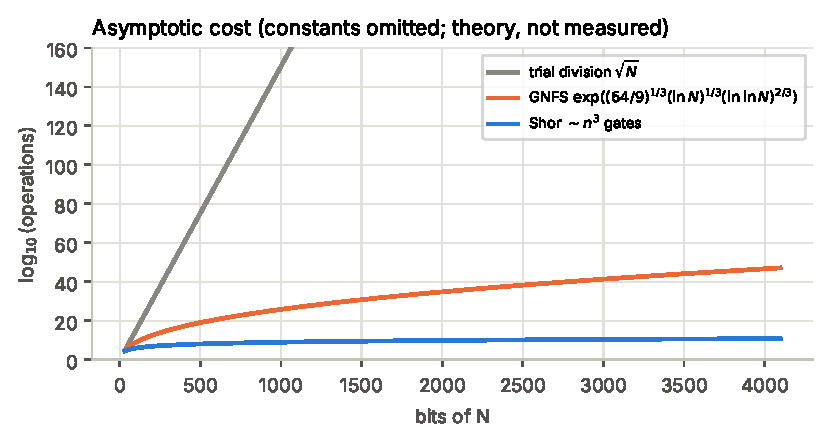
\includegraphics[width=\linewidth]{complexity.pdf}
      {\scriptsize\color{qgrey} \tagtheory{} asymptotic formulas with constants omitted --- not measured run times.}
    \end{column}
    \begin{column}{0.38\textwidth}
      \footnotesize
      \begin{tabular}{@{}ll@{}}
        \toprule method & cost ($n$ bits) \\ \midrule
        trial division & $2^{n/2}$ \\
        Pollard rho & $2^{n/4}$ \\
        GNFS & $e^{1.92\,n^{1/3}(\ln n)^{2/3}}$ \\
        Shor & $O(n^3)$ \\ \bottomrule
      \end{tabular}\\[4pt]
      \small Doubling $n$ multiplies Shor's gate count by $8$; for GNFS the cost grows faster than any polynomial.
    \end{column}
  \end{columns}
\end{frame}

\begin{frame}[label=fRSAdep]{Why RSA relies on factoring}
  \begin{columns}[T]
    \begin{column}{0.5\textwidth}
      \small
      \begin{enumerate}\itemsep1pt
        \item choose primes $p, q$; publish $N = pq$ and $e$
        \item secret $d = e^{-1} \bmod \varphi(N)$, $\varphi(N) = (p - 1)(q - 1)$
        \item encrypt $c = m^e \bmod N$, decrypt $m = c^d \bmod N$
      \end{enumerate}
      Knowing $p, q$ $\Rightarrow$ $\varphi(N)$ $\Rightarrow$ $d$: \hl{factoring breaks RSA}.
    \end{column}
    \begin{column}{0.46\textwidth}
      \begin{exampleblock}{Toy RSA}
        \small $p = 5$, $q = 11$, $N = 55$, $\varphi = 40$, $e = 7$\\
        $d = 23$ ($7\cdot23 = 161 \equiv 1 \bmod 40$)\\
        $m = 2$: $c = 2^7 \bmod 55 = 18$; $18^{23} \bmod 55 = 2$ \checkmark
      \end{exampleblock}
      \scriptsize\color{qgrey} Real RSA uses $\ge 2048$-bit $N$ with padding; the toy example only shows the algebra.
    \end{column}
  \end{columns}
\end{frame}

% =====================================================================================
\section{Module 4: Core idea}
\begin{frame}[label=fReduction]{Reduction of factoring to order finding}
  \centering
  \resizebox{\linewidth}{!}{%
  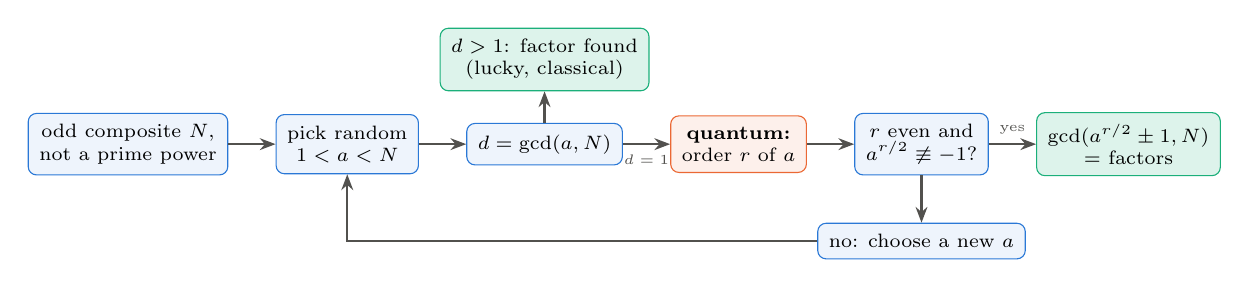
\begin{tikzpicture}[node distance=4mm and 6mm]
    \node[box] (n) {odd composite $N$,\\ not a prime power};
    \node[box, right=of n] (a) {pick random\\ $1 < a < N$};
    \node[box, right=of a] (g) {$d = \gcd(a, N)$};
    \node[box, fill=qaqua!15, draw=qaqua, above=4mm of g] (lucky) {$d > 1$: factor found\\ (lucky, classical)};
    \node[qbox, right=of g] (q) {\textbf{quantum:}\\ order $r$ of $a$};
    \node[box, right=of q] (chk) {$r$ even and\\ $a^{r/2} \not\equiv -1$?};
    \node[box, fill=qaqua!15, draw=qaqua, right=of chk] (f) {$\gcd(a^{r/2} \pm 1, N)$\\ = factors};
    \node[box, below=6mm of chk] (rep) {no: choose a new $a$};
    \draw[arr] (n) -- (a); \draw[arr] (a) -- (g); \draw[arr] (g) -- (lucky); \draw[arr] (g) -- node[below, font=\tiny]{$d = 1$} (q);
    \draw[arr] (q) -- (chk); \draw[arr] (chk) -- node[above, font=\tiny]{yes} (f); \draw[arr] (chk) -- (rep); \draw[arr] (rep) -| (a);
  \end{tikzpicture}}
  \vspace{4pt}
  \begin{block}{Only one step is quantum}
    \small Everything except ``order $r$ of $a$'' runs on a classical computer in polynomial time. For random $a$ the test succeeds with probability
    $\ge 1 - 2^{-(k-1)} \ge \frac12$ ($k$ = number of distinct prime factors), so a few repetitions suffice.
  \end{block}
\end{frame}

\begin{frame}[label=fPeriodic]{The periodic function $f(x) = a^x \bmod N$}
  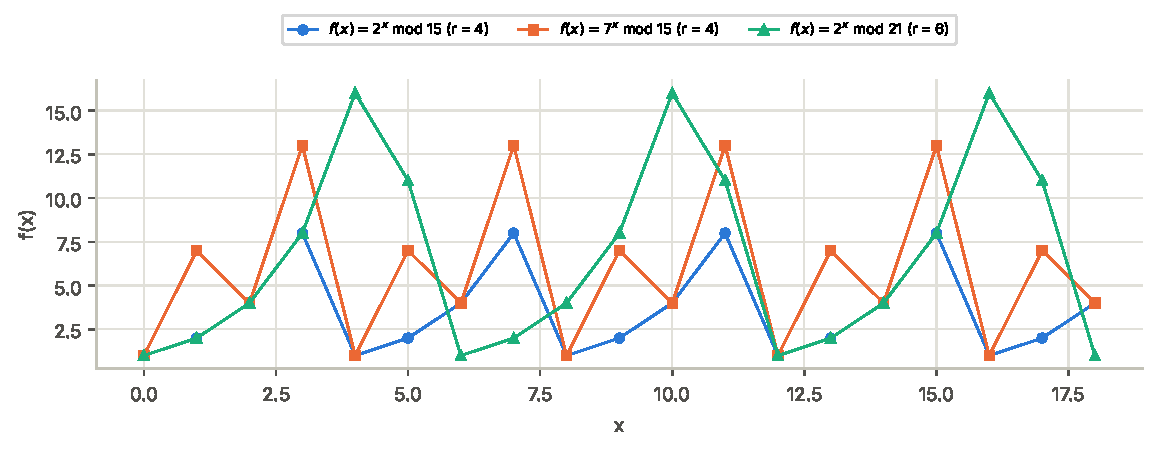
\includegraphics[width=\linewidth]{periodic.pdf}
  \small
  \begin{columns}[T]
    \begin{column}{0.5\textwidth}
      $2^x \bmod 15$: $1, 2, 4, 8, 1, 2, 4, 8, \dots$ $\Rightarrow r = 4$\\
      $7^x \bmod 15$: $1, 7, 4, 13, 1, \dots$ $\Rightarrow r = 4$
    \end{column}
    \begin{column}{0.46\textwidth}
      $2^x \bmod 21$: $1, 2, 4, 8, 16, 11, 1, \dots$ $\Rightarrow r = 6$\\
      {\color{qgrey}\scriptsize The values look random inside one period; only the repetition carries information.}
    \end{column}
  \end{columns}
\end{frame}

\begin{frame}[label=fWhyEven]{Why $r$ must be even and $a^{r/2} \not\equiv -1$}
  \begin{columns}[T]
    \begin{column}{0.52\textwidth}
      \small
      $a^r \equiv 1 \Rightarrow (a^{r/2} - 1)(a^{r/2} + 1) \equiv 0 \pmod N$ --- needs $r$ \key{even}.
      \begin{itemize}\itemsep1pt
        \item $a^{r/2} \not\equiv 1$ always (else the order would be $r/2$)
        \item if $a^{r/2} \equiv -1$: $N \mid a^{r/2} + 1$, gcds $N$ and $1$ --- \hl{trivial}
        \item otherwise $N$ divides the product but neither factor $\Rightarrow$
      \end{itemize}
      \[ p = \gcd(a^{r/2} - 1, N),\qquad q = \gcd(a^{r/2} + 1, N) \]
    \end{column}
    \begin{column}{0.44\textwidth}
      \begin{exampleblock}{Cases}
        \scriptsize
        \begin{tabular}{@{}llll@{}}
          $N, a$ & $r$ & $a^{r/2}$ & result\\ \midrule
          $15, 2$ & $4$ & $4$ & $3\times5$ \checkmark\\
          $15, 14$ & $2$ & $14 \equiv -1$ & trivial \ding{55}\\
          $21, 4$ & $3$ & --- & odd \ding{55}\\
          $21, 5$ & $6$ & $20 \equiv -1$ & trivial \ding{55}\\
          $21, 2$ & $6$ & $8$ & $7\times3$ \checkmark\\
          $21, 6$ & --- & --- & $\gcd = 3$ (lucky)
        \end{tabular}
      \end{exampleblock}
      \scriptsize\color{qgrey} A failed attempt is a failure: report it and repeat with another $a$.
    \end{column}
  \end{columns}
\end{frame}

\begin{frame}[label=fPrimePower]{When the reduction does not apply}
  \small
  \begin{itemize}\itemsep3pt
    \item \key{$N$ even}: factor $2$ immediately.
    \item \key{$N$ prime}: nothing to factor (fast primality tests).
    \item \key{$N = p^k$ a prime power}: $\mathbb Z_{p^k}^*$ is cyclic, so the only square roots of $1$ are $\pm1$ and $\gcd(a^{r/2} \pm 1, N)$ is always trivial.
          Detected classically by integer $k$-th roots (\texttt{prime\_power} in the notebook).
    \item \key{$N$ with $k \ge 2$ distinct odd prime factors}: at least a fraction $1 - 2^{-(k-1)}$ of the bases works.
  \end{itemize}
  \begin{block}{\tagimpl{} \texttt{Shor.ipynb}}
    \small handles even $N$, primes and prime powers classically before any quantum computation; invalid or lucky bases are reported and replaced
    by a random $a$; failed attempts are retried up to \texttt{MAX\_ATTEMPTS} times.
  \end{block}
\end{frame}

% =====================================================================================
\section{Module 5: Quantum foundations}
\begin{frame}[label=fRegisters]{Qubits and registers --- in the language of Shor}
  \begin{columns}[T]
    \begin{column}{0.52\textwidth}
      \small
      \begin{itemize}\itemsep1pt
        \item A register of $m$ qubits holds a superposition of the integers $0, \dots, 2^m - 1$: $\sum_x\alpha_x\ket x$.
        \item \key{Counting (input) register}: $t$ qubits for the exponent $x$; in the notebook $t = 2n$.
        \item \key{Work (function) register}: $n$ qubits for values mod $N$, initialised to $\ket1$.
        \item Total: $t + n = 3n$ qubits; $n = $ \texttt{N.bit\_length()}.
      \end{itemize}
    \end{column}
    \begin{column}{0.44\textwidth}
      \begin{exampleblock}{Register sizes (notebook)}
        \scriptsize
        \begin{tabular}{@{}rrrr@{}}
          $N$ & $n$ & $t$ & qubits\\ \midrule
          15 & 4 & 8 & 12\\
          21 & 5 & 10 & 15\\
          33, 35 & 6 & 12 & 18\\
          143 & 8 & 16 & 24
        \end{tabular}
      \end{exampleblock}
      \scriptsize Integers are stored in binary: $\ket{0001} = \ket1$; the notebook puts the least significant bit on the \emph{last} work qubit.
    \end{column}
  \end{columns}
\end{frame}

\begin{frame}[label=fSuperposition]{Superposition, Hadamard gates and quantum parallelism}
  \begin{columns}[T]
    \begin{column}{0.52\textwidth}
      \small
      \[ H\ket0 = \tfrac{1}{\sqrt2}(\ket0 + \ket1),\qquad H^{\otimes t}\ket{0}^{\otimes t} = \tfrac{1}{\sqrt{2^t}}\sum_{x=0}^{2^t-1}\ket x \]
      A reversible circuit $U_f$ then gives
      \[ \tfrac{1}{\sqrt{2^t}}\sum_x\ket x\ket{f(x)} \quad\text{(``all $x$ at once'')} \]
    \end{column}
    \begin{column}{0.44\textwidth}
      \begin{alertblock}{Parallelism is not enough}
        \small Measuring this state returns \emph{one} random pair $(x, f(x))$ --- no better than one classical evaluation. The period is hidden in the
        \key{amplitudes}; extracting it needs \hl{interference}.
      \end{alertblock}
      \scriptsize $t = 8$: each $\ket x$ has amplitude $1/16$, probability $1/256$.
    \end{column}
  \end{columns}
\end{frame}

\begin{frame}[label=fGates]{Unitary, reversible and controlled gates}
  \begin{columns}[T]
    \begin{column}{0.5\textwidth}
      \small
      \begin{itemize}\itemsep1pt
        \item Gates are \key{unitary}: $U^\dagger U = I$, hence \key{reversible}.
        \item $x \mapsto a^x \bmod N$ is \hl{not} injective ($x$ and $x + r$ collide) $\Rightarrow$ keep $x$: $\ket x\ket1 \mapsto \ket x\ket{a^x \bmod N}$.
        \item $U_a\ket y = \ket{ay \bmod N}$ ($y < N$) is a \key{permutation} for $\gcd(a, N) = 1$ $\Rightarrow$ unitary.
        \item \key{Controlled-$U$}: apply $U$ only on the $\ket1$ branch of a control qubit.
      \end{itemize}
    \end{column}
    \begin{column}{0.46\textwidth}
      \centering
      \begin{quantikz}[row sep=0.25cm, column sep=0.3cm]
        \lstick{control} & \ctrl{1} & \qw \\
        \lstick{$\ket y$} & \gate{U_a} & \qw \rstick{$\ket{a^cy \bmod N}$}
      \end{quantikz}\\[4pt]
      \scriptsize Phase gate $R_1(\lambda) = \operatorname{diag}(1, e^{i\lambda})$: $R_1(\pi) = Z$, $R_1(\frac\pi2) = S$, $R_1(\frac\pi4) = T$.
      Controlled $R_1$ gates build the QFT.
    \end{column}
  \end{columns}
\end{frame}

\begin{frame}[label=fEntangle]{Entanglement, measurement and interference}
  \begin{columns}[T]
    \begin{column}{0.5\textwidth}
      \small
      \key{Entanglement}: after modular exponentiation the registers are correlated,
      \[ \tfrac{1}{\sqrt8}\sum_{x=0}^{7}\ket x\ket{2^x \bmod 15} = \tfrac{1}{\sqrt8}\big(\ket0\ket1 + \ket1\ket2 + \ket2\ket4 + \dots\big) \]
      \key{Measurement} of the work register with result $4$ ($P = 1/4$) leaves $\frac{1}{\sqrt2}(\ket2 + \ket6)$: periodic, period $4$, random offset.
    \end{column}
    \begin{column}{0.46\textwidth}
      \key{Interference}: amplitudes of paths add \emph{before} squaring:
      \[ \big|\tfrac12 + \tfrac12e^{i\theta}\big|^2 = \cos^2\tfrac\theta2 \]
      \small constructive for $\theta = 0$, destructive for $\theta = \pi$. The inverse QFT arranges the phases so that only $y \approx k2^t/r$ survive.
      \begin{block}{Implicit measurement}
        \scriptsize Measuring the work register is not necessary: the distribution of $y$ is the same (the notebook measures only the counting register).
      \end{block}
    \end{column}
  \end{columns}
\end{frame}

% =====================================================================================
\section{Module 6: Quantum period finding}
\begin{frame}[label=fPFCircuit]{The period-finding (order-finding) circuit}
  \centering
  \begin{quantikz}[row sep=0.22cm, column sep=0.32cm]
    \lstick{$\ket0$ \scriptsize($x_2$, MSB)} & \gate{H} & \qw & \qw & \ctrl{3} & \gate[3]{\mathrm{QFT}^{-1}} & \meter{} \\
    \lstick{$\ket0$ \scriptsize($x_1$)} & \gate{H} & \qw & \ctrl{2} & \qw & & \meter{} \\
    \lstick{$\ket0$ \scriptsize($x_0$, LSB)} & \gate{H} & \ctrl{1} & \qw & \qw & & \meter{} \\
    \lstick{$\ket1$ \scriptsize(work, $n$ qubits)} & \qwbundle{n} & \gate{U_a} & \gate{U_{a^2}} & \gate{U_{a^4}} & \qw & \qw
  \end{quantikz}\\[4pt]
  \small
  \begin{enumerate}\itemsep0pt
    \item Hadamards: uniform superposition over the exponent $x$ ($t = 3$ shown; the notebook uses $t = 2n$)
    \item controlled $U_{a^{2^j}}$ on qubit $x_j$: together $\ket x\ket1 \mapsto \ket x\ket{a^x \bmod N}$ (repeated squaring)
    \item inverse QFT on the counting register, measure $y$; classical post-processing gives $r$
  \end{enumerate}
\end{frame}

\begin{frame}[label=fPFState]{State after each step}
  \small
  \begin{align*}
    \ket{\psi_0} &= \ket{0}^{\otimes t}\ket1\\
    \ket{\psi_1} &= \frac{1}{\sqrt{2^t}}\sum_{x=0}^{2^t-1}\ket x\ket1 && \text{(Hadamards)}\\
    \ket{\psi_2} &= \frac{1}{\sqrt{2^t}}\sum_{x=0}^{2^t-1}\ket x\ket{a^x \bmod N} = \frac{1}{\sqrt{2^t}}\sum_{v}\Big(\sum_{x:\,a^x \equiv v}\ket x\Big)\ket v && \text{(group by value)}\\
    \ket{\psi_3} &= \sum_y\Big(\frac{1}{2^t}\sum_x e^{-2\pi ixy/2^t}\ket y\Big)\ket{a^x} && \text{(inverse QFT)}
  \end{align*}
  For each value $v$ the $x$'s form an arithmetic progression $x_0, x_0 + r, x_0 + 2r, \dots$ The geometric sum $\sum_me^{-2\pi imry/2^t}$ is large only when
  $ry/2^t$ is close to an integer, i.e.\ \hl{$y \approx k\cdot2^t/r$}. The offset $x_0$ only adds a phase.
\end{frame}

\begin{frame}[label=fPFExact]{When $r$ divides $2^t$: exact peaks}
  \begin{columns}[T]
    \begin{column}{0.5\textwidth}
      \small
      If $r \mid 2^t$, each progression has exactly $M = 2^t/r$ terms and
      \[ \Big|\sum_{m=0}^{M-1}e^{-2\pi imry/2^t}\Big|^2 = \begin{cases}M^2 & y = k2^t/r\\ 0 & \text{otherwise}\end{cases} \]
      so $P(y = k2^t/r) = 1/r$ for $k = 0, \dots, r - 1$.
    \end{column}
    \begin{column}{0.46\textwidth}
      \begin{exampleblock}{$N = 15$, $a = 7$ (or $2$), $t = 8$}
        \small $r = 4$: outcomes $0, 64, 128, 192$, each with probability exactly $1/4$.
      \end{exampleblock}
      \begin{exampleblock}{$N = 15$, $a = 11$}
        \small $r = 2$: outcomes $0, 128$, each $1/2$.
      \end{exampleblock}
      \scriptsize\color{qgrey} For $r \nmid 2^t$ (e.g.\ $N = 21$, $r = 6$) the peaks have finite width --- next modules.
    \end{column}
  \end{columns}
\end{frame}

\begin{frame}[label=fPFIntuition]{Intuition: a quantum ``frequency analyser''}
  \small
  \begin{columns}[T]
    \begin{column}{0.5\textwidth}
      \begin{itemize}\itemsep2pt
        \item The counting register holds a \key{comb} with spacing $r$: $\ket{x_0} + \ket{x_0 + r} + \ket{x_0 + 2r} + \cdots$
        \item The Fourier transform of a comb with spacing $r$ is a comb with spacing $2^t/r$ --- like a discrete Fourier transform of a periodic signal.
        \item Measuring after the transform samples a random \key{frequency} $k/r$.
      \end{itemize}
    \end{column}
    \begin{column}{0.46\textwidth}
      \begin{block}{Why this is fast}
        \small The QFT on $t$ qubits needs only $O(t^2)$ gates, while the classical FFT of the $2^t$ amplitudes would need $O(t\,2^t)$ operations ---
        but the quantum version gives only \emph{samples}, which is all we need.
      \end{block}
    \end{column}
  \end{columns}
\end{frame}

% =====================================================================================
\section{Module 7: QFT in Shor's algorithm}
\begin{frame}[label=fQFTDef]{The quantum Fourier transform}
  \begin{columns}[T]
    \begin{column}{0.52\textwidth}
      \small
      \[ \mathrm{QFT}\ket x = \frac{1}{\sqrt{2^t}}\sum_{y=0}^{2^t-1}e^{2\pi ixy/2^t}\ket y \]
      Product form (the key to an efficient circuit):
      \[ \mathrm{QFT}\ket{x} = \bigotimes_{l=1}^{t}\frac{\ket0 + e^{2\pi i\,0.x_{l-1}\cdots x_0}\ket1}{\sqrt2} \]
      The inverse QFT has the conjugate phases, $e^{-2\pi ixy/2^t}$.
    \end{column}
    \begin{column}{0.44\textwidth}
      \begin{block}{Why Shor needs it}
        \small It converts the \key{period} $r$ of the comb into \key{peaks} at multiples of $2^t/r$ that a single measurement can sample.
      \end{block}
      \begin{alertblock}{Common mistake}
        \small The QFT is \hl{not} Shor's algorithm. Without modular exponentiation and classical post-processing it factors nothing.
        See the companion QFT lecture for full details.
      \end{alertblock}
    \end{column}
  \end{columns}
\end{frame}

\begin{frame}[label=fQFTCircuit]{QFT circuit: Hadamards and controlled phase rotations}
  \centering
  \begin{quantikz}[row sep=0.25cm, column sep=0.3cm]
    \lstick{$x_2$} & \gate{H} & \gate{R_2} & \gate{R_3} & \qw & \qw & \qw & \swap{2} & \qw\\
    \lstick{$x_1$} & \qw & \ctrl{-1} & \qw & \gate{H} & \gate{R_2} & \qw & \qw & \qw\\
    \lstick{$x_0$} & \qw & \qw & \ctrl{-2} & \qw & \ctrl{-1} & \gate{H} & \targX{} & \qw
  \end{quantikz}\\[4pt]
  \small $R_k = R_1(2\pi/2^k)$. For $t$ qubits: $t$ Hadamards, $t(t - 1)/2$ controlled phases, $\lfloor t/2\rfloor$ SWAPs: $O(t^2)$ gates.
  \begin{block}{Inverse QFT in \texttt{Shor.ipynb} \tagimpl}
    \small the mirror image: SWAPs first, then for each qubit the controlled phases \texttt{cr1(-pi/2**(k-j))} followed by \texttt{h}. For $t = 8$: 4 SWAPs,
    $28$ controlled phases, $8$ Hadamards.
  \end{block}
\end{frame}

\begin{frame}[label=fQFTPeaks]{From periodic states to Fourier peaks}
  \begin{columns}[T]
    \begin{column}{0.5\textwidth}
      \small
      Comb of $M$ teeth, spacing $r$, offset $x_0$:
      \[ P(y) = \frac{1}{2^tM}\Big|\sum_{m=0}^{M-1}e^{-2\pi imry/2^t}\Big|^2 = \frac{\sin^2(\pi Mry/2^t)}{2^tM\sin^2(\pi ry/2^t)} \]
      Peaks at $y \approx k2^t/r$; the \key{nearest} integer to each peak gets probability $\ge 4/\pi^2 \cdot \frac1r$.
    \end{column}
    \begin{column}{0.46\textwidth}
      \begin{block}{Measurement outcome}
        \small $y/2^t \approx k/r$ with \key{random} $k \in \{0, \dots, r - 1\}$. Neither $k$ nor $r$ is known --- only the ratio, approximately.
      \end{block}
      \begin{exampleblock}{$N = 21$, $a = 2$, $t = 10$}
        \small $2^{10}/6 = 170.67$: peaks near $0, 171, 341, 512, 683, 853$; $P(171) = \numpeaktwentyone$, $P(0) = P(512) = 1/6$.
      \end{exampleblock}
    \end{column}
  \end{columns}
\end{frame}

\begin{frame}[label=fQFTRole]{What the QFT does --- and does not do --- in Shor's algorithm}
  \small
  \begin{columns}[T]
    \begin{column}{0.48\textwidth}
      \begin{block}{Does}
        \begin{itemize}\itemsep1pt
          \item turns periodicity into frequency peaks
          \item decodes the binary phase pattern of phase estimation
          \item costs only $O(t^2)$ gates (fewer when approximated)
        \end{itemize}
      \end{block}
    \end{column}
    \begin{column}{0.48\textwidth}
      \begin{alertblock}{Does not}
        \begin{itemize}\itemsep1pt
          \item compute $a^x \bmod N$ (the expensive part)
          \item output $r$ directly (continued fractions needed)
          \item output the factors (gcds needed)
        \end{itemize}
      \end{alertblock}
    \end{column}
  \end{columns}
  \vspace{4pt}
  \centering\color{qgrey} Shor $=$ classical reduction $+$ \{superposition, modular exponentiation, inverse QFT, measurement\} $+$ classical post-processing.
\end{frame}

% =====================================================================================
\section{Module 8: Quantum phase estimation}
\begin{frame}[label=fEigen]{Eigenvalues and eigenvectors of $U_a$}
  \begin{columns}[T]
    \begin{column}{0.52\textwidth}
      \small
      On the orbit $\ket1 \to \ket a \to \ket{a^2} \to \dots \to \ket1$, $U_a$ is a cyclic shift of length $r$. Its eigenvectors are
      \[ \ket{u_s} = \frac{1}{\sqrt r}\sum_{k=0}^{r-1}e^{-2\pi isk/r}\ket{a^k \bmod N} \]
      \[ U_a\ket{u_s} = e^{2\pi is/r}\ket{u_s},\qquad s = 0, \dots, r - 1 \]
      \key{The order is in the eigenphases} $s/r$.
    \end{column}
    \begin{column}{0.44\textwidth}
      \begin{exampleblock}{$U_2$ modulo 15}
        \small orbit $1 \to 2 \to 4 \to 8 \to 1$, eigenvalues $1, i, -1, -i$
      \end{exampleblock}
      \begin{block}{Trick: no eigenvector needed}
        \small $\frac{1}{\sqrt r}\sum_{s=0}^{r-1}\ket{u_s} = \ket1$. Starting the work register in $\ket1$ runs phase estimation on a \emph{uniformly random} eigenvector.
      \end{block}
    \end{column}
  \end{columns}
\end{frame}

\begin{frame}[label=fKickback]{Phase kickback}
  \begin{columns}[T]
    \begin{column}{0.5\textwidth}
      \centering
      \begin{quantikz}[row sep=0.3cm, column sep=0.35cm]
        \lstick{$\ket+$} & \ctrl{1} & \qw \rstick{$\frac{\ket0 + e^{i\phi}\ket1}{\sqrt2}$}\\
        \lstick{$\ket u$} & \gate{U} & \qw \rstick{$\ket u$}
      \end{quantikz}\\[6pt]
      \small $U\ket u = e^{i\phi}\ket u$: the target is \hl{unchanged}; the phase moves to the $\ket1$ branch of the \key{control}.
    \end{column}
    \begin{column}{0.46\textwidth}
      \small
      \begin{itemize}\itemsep2pt
        \item $\langle X\rangle$ of the control $= \cos\phi$: for $\phi = 2\pi/3$, $-\frac12$.
        \item $U^{2^j}$ kicks back $2^j\phi$: counting qubit $j$ stores the phase doubled $j$ times.
        \item ``Controlled gates never change the control'' is \hl{false} in quantum computing.
      \end{itemize}
    \end{column}
  \end{columns}
\end{frame}

\begin{frame}[label=fQPE]{Quantum phase estimation (QPE)}
  \begin{columns}[T]
    \begin{column}{0.55\textwidth}
      \small
      After the controlled $U^{2^j}$ gates the counting register is
      \[ \bigotimes_j\frac{\ket0 + e^{2\pi i2^j\varphi}\ket1}{\sqrt2} = \frac{1}{\sqrt{2^t}}\sum_xe^{2\pi ix\varphi}\ket x \]
      --- exactly $\mathrm{QFT}\ket{2^t\varphi}$ when $2^t\varphi$ is an integer. The inverse QFT returns $y \approx 2^t\varphi$:
      \[ P(y) = \Big|\frac{1}{2^t}\sum_xe^{2\pi ix(\varphi - y/2^t)}\Big|^2 \]
    \end{column}
    \begin{column}{0.41\textwidth}
      \begin{exampleblock}{$t = 3$}
        \small
        $\varphi = 3/8$: $y = 3$ with probability $1$.\\
        $\varphi = 1/3$: $y = 3$ with $P \approx 0.69$, $y = 2$ with $0.17$.
      \end{exampleblock}
      \scriptsize The nearest outcome always has $P \ge 4/\pi^2 \approx 0.405$; more counting qubits sharpen the peak.
    \end{column}
  \end{columns}
\end{frame}

\begin{frame}[label=fQPEOrder]{Order finding $=$ phase estimation of $U_a$}
  \small
  \begin{columns}[T]
    \begin{column}{0.5\textwidth}
      \begin{itemize}\itemsep2pt
        \item eigenphase $\varphi = s/r$ with $s$ uniform in $\{0, \dots, r - 1\}$
        \item measured $y \approx 2^t s/r$ --- the \emph{same} peaks as in the period-finding picture
        \item controlled $U_a^{2^j} = U_{a^{2^j} \bmod N}$: the constants are precomputed classically
      \end{itemize}
    \end{column}
    \begin{column}{0.46\textwidth}
      \begin{block}{Two views, one circuit}
        \scriptsize
        \begin{tabular}{@{}p{0.45\linewidth}p{0.45\linewidth}@{}}
          \textbf{period finding} & \textbf{phase estimation}\\
          comb in $x$ with spacing $r$ & eigenphases $s/r$\\
          measure work register (optional) & work register in $\ket1$\\
          Fourier peaks $k2^t/r$ & $y \approx 2^ts/r$
        \end{tabular}
      \end{block}
    \end{column}
  \end{columns}
  \vspace{2pt}
  \centering The QPE view explains why $t \approx 2n$ counting qubits are used: the phase must be resolved to precision $\approx 1/N^2$.
\end{frame}

% =====================================================================================
\section{Module 9: Continued fractions}
\begin{frame}[label=fCFWhy]{Why the measurement does not give $r$ directly}
  \small
  \begin{itemize}\itemsep2pt
    \item The outcome $y$ is \key{random}: we learn $y/2^t \approx s/r$ for a random $s$.
    \item $s/r$ may not be in lowest terms: if $\gcd(s, r) > 1$ we only see a \key{divisor} of $r$.
    \item $y = 0$ ($s = 0$) occurs for every $r$ and carries \hl{no} information.
    \item When $r \nmid 2^t$, $y$ is only close to $2^ts/r$; neighbouring values also occur.
  \end{itemize}
  \begin{block}{Goal of post-processing}
    \small find the fraction $s/r$ with $r \le N$ closest to $y/2^t$, then \key{verify} $a^r \equiv 1$ classically --- the quantum computer only proposes candidates.
  \end{block}
\end{frame}

\begin{frame}[label=fCF]{Continued fractions}
  \begin{columns}[T]
    \begin{column}{0.52\textwidth}
      \small
      \[ x = a_0 + \cfrac{1}{a_1 + \cfrac{1}{a_2 + \cdots}} = [a_0; a_1, a_2, \dots] \]
      Algorithm: $a_0 = \lfloor x\rfloor$, repeat on $1/(x - a_0)$. Truncations are the \key{convergents} --- the best rational approximations.
      \begin{block}{Legendre's theorem}
        \scriptsize If $\big|\frac{y}{2^t} - \frac sr\big| < \frac{1}{2r^2}$, then $s/r$ is a convergent of $y/2^t$. With $2^t \ge N^2$ the nearest outcome satisfies this.
      \end{block}
    \end{column}
    \begin{column}{0.44\textwidth}
      \begin{exampleblock}{$y = 171$, $t = 10$, $N = 21$}
        \small
        $171/1024 = [0; 5, 1, 84, 2]$\\
        convergents: $0,\ \frac15,\ \frac16,\ \frac{85}{511}, \dots$\\
        largest denominator $\le 21$: $\mathbf{1/6}$ $\Rightarrow$ $r = 6$\\
        check: $2^6 = 64 \equiv 1 \pmod{21}$ \checkmark
      \end{exampleblock}
      \scriptsize In Python: \texttt{Fraction(171, 1024).limit\_denominator(21)} $\to$ \texttt{Fraction(1, 6)}.
    \end{column}
  \end{columns}
\end{frame}

\begin{frame}[label=fCFTable]{Post-processing the likely outcomes for $N = 21$, $a = 2$ \tagillus}
  \centering
  \resizebox{0.9\linewidth}{!}{% GENERATED by make_figures.py - do not edit
\begin{tabular}{rrrlllr}\toprule
$y$ & $P(y)$ & $y/2^{10}$ & continued fraction & $s/r$ & $r$ & factors \\ \midrule
0 & 0.1667 & 0.00000 & $[0]$ & - & - & none \\
170 & 0.0285 & 0.16602 & $[0;6;42;2]$ & $1/6$ & 6 & $3\times7$ \\
171 & 0.1140 & 0.16699 & $[0;5;1;84;2]$ & $1/6$ & 6 & $3\times7$ \\
341 & 0.1140 & 0.33301 & $[0;3;341]$ & $1/3$ & 6 & $3\times7$ \\
342 & 0.0285 & 0.33398 & $[0;2;1;170]$ & $1/3$ & 6 & $3\times7$ \\
512 & 0.1667 & 0.50000 & $[0;2]$ & $1/2$ & 6 & $3\times7$ \\
683 & 0.1140 & 0.66699 & $[0;1;2;341]$ & $2/3$ & 6 & $3\times7$ \\
853 & 0.1140 & 0.83301 & $[0;1;4;1;84;2]$ & $5/6$ & 6 & $3\times7$ \\
\bottomrule
\end{tabular}
}\\[4pt]
  \small Exact probabilities from the CUDA-Q state vector of the notebook's circuit ($t = 10$). $y = 512$ gives $1/2$; the \key{multiples test}
  ($2, 4, 6$) recovers $r = 6$. $y = 0$ gives nothing. In total $P_{\text{succ}} = \numsucctwentyonetwo$ per shot.
\end{frame}

\begin{frame}[fragile,label=fCFCode]{Verifying the candidate and recovering the factors \tagimpl}
  \begin{columns}[T]
    \begin{column}{0.54\textwidth}
\begin{lstlisting}
def candidate_orders(y, t, modulus, a):
    if y == 0:
        return None, []
    fraction = Fraction(y, 2 ** t)
    fraction = fraction.limit_denominator(modulus)
    base = fraction.denominator
    return fraction, [base * k for k in
        range(1, modulus // base + 1)
        if pow(a, base * k, modulus) == 1][:1]
\end{lstlisting}
      \scriptsize\color{qgrey} Copied from \texttt{Shor.ipynb} (Section 7a).
    \end{column}
    \begin{column}{0.4\textwidth}
      \small
      \begin{enumerate}\itemsep1pt
        \item denominator $r'$ of the closest fraction
        \item smallest multiple $kr'$ with $a^{kr'} \equiv 1$ (repairs $\gcd(s, r) > 1$)
        \item $r$ even, $x = a^{r/2} \not\equiv -1$
        \item $p = \gcd(x - 1, N)$, $q = \gcd(x + 1, N)$
        \item check $p\cdot q = N$
      \end{enumerate}
      Without step 2 a shot succeeds with probability about $\varphi(r)/r$.
    \end{column}
  \end{columns}
\end{frame}

% =====================================================================================
\section{Module 10: Worked examples}
\begin{frame}[label=fEx15a]{Factoring $N = 15$ with $a = 2$: classical steps 1--4}
  \begin{columns}[T]
    \begin{column}{0.5\textwidth}
      \small
      \begin{enumerate}\itemsep2pt
        \item $\gcd(2, 15) = 1$ --- no lucky factor; continue.
        \item $f(x) = 2^x \bmod 15$.
        \item values:\\[2pt]
          {\scriptsize\begin{tabular}{c|cccccccc}
            $x$ & 0 & 1 & 2 & 3 & 4 & 5 & 6 & 7\\ \hline
            $f$ & 1 & 2 & 4 & 8 & 1 & 2 & 4 & 8
          \end{tabular}}
        \item period $r = 4$ --- \hl{read off here only because $N$ is tiny}; for large $N$ this table is impossible to compute.
      \end{enumerate}
    \end{column}
    \begin{column}{0.46\textwidth}
      \begin{alertblock}{Mathematical example, not a hardware run}
        \small Steps 3--4 are what the quantum computer replaces. In this lecture the quantum part was \emph{simulated} on a CPU; no quantum device was used.
      \end{alertblock}
      \scriptsize Registers (notebook): $n = 4$, $t = 8$, 12 qubits.
    \end{column}
  \end{columns}
\end{frame}

\begin{frame}[label=fEx15b]{$N = 15$, $a = 2$: the quantum part (steps 5--6)}
  \small
  \begin{columns}[T]
    \begin{column}{0.55\textwidth}
      \begin{align*}
        &\tfrac{1}{16}\textstyle\sum_{x=0}^{255}\ket x\ket1 \xrightarrow{\ U\ } \tfrac{1}{16}\textstyle\sum_x\ket x\ket{2^x \bmod 15}\\
        &= \tfrac12\big(\ket{c_1}\ket1 + \ket{c_2}\ket2 + \ket{c_4}\ket4 + \ket{c_8}\ket8\big)
      \end{align*}
      with combs $\ket{c_v} = \frac18\sum_{m=0}^{63}\ket{x_0 + 4m}$. The inverse QFT maps each comb to peaks at $y \in \{0, 64, 128, 192\}$, each
      with probability $1/4$.
    \end{column}
    \begin{column}{0.41\textwidth}
      \begin{block}{Controlled multiplications}
        \small $2^{2^j} \bmod 15$: $2, 4, 1, 1, \dots$ --- only $U_2$ and $U_4$ are non-trivial (counting qubits $x_0$ and $x_1$).
      \end{block}
      \begin{exampleblock}{\tagillus{} re-executed}
        \scriptsize 1000 shots, seed 42: 4 distinct outcomes, success fraction $\numshotfifteentwo$ (exact $\numsuccfifteentwo$).
      \end{exampleblock}
    \end{column}
  \end{columns}
\end{frame}

\begin{frame}[label=fEx15c]{$N = 15$, $a = 2$: post-processing and verification (steps 7--12)}
  \footnotesize
  \begin{center}
  \begin{tabular}{rcccl}
    \toprule $y$ & $y/256$ & fraction & candidate $r$ & result \\ \midrule
    0 & 0 & --- & --- & no information (probability $1/4$) \\
    64 & 0.25 & $1/4$ & 4 & $2^4 = 16 \equiv 1$ \checkmark \\
    128 & 0.5 & $1/2$ & $2 \to$ multiples $\to 4$ & $2^2 = 4 \ne 1$, $2^4 \equiv 1$ \checkmark\\
    192 & 0.75 & $3/4$ & 4 & \checkmark \\ \bottomrule
  \end{tabular}
  \end{center}
  \small
  \begin{columns}[T]
    \begin{column}{0.5\textwidth}
      \begin{itemize}\itemsep1pt
        \item[8.] verified $r = 4$: even, $2^{r/2} = 4 \not\equiv 14$
        \item[9.] $\gcd(4 - 1, 15) = \gcd(3, 15) = \mathbf{3}$
        \item[10.] $\gcd(4 + 1, 15) = \gcd(5, 15) = \mathbf{5}$
      \end{itemize}
    \end{column}
    \begin{column}{0.46\textwidth}
      \begin{itemize}\itemsep1pt
        \item[11.] non-trivial factors $3$ and $5$
        \item[12.] $3 \times 5 = 15$ \checkmark
      \end{itemize}
      Success per shot: $3/4$ (only $y = 0$ fails).
    \end{column}
  \end{columns}
\end{frame}

\begin{frame}[label=fEx21]{Second example: $N = 21$, $a = 2$ ($r = 6$ does not divide $2^t$)}
  \begin{columns}[T]
    \begin{column}{0.5\textwidth}
      \small
      \begin{enumerate}\itemsep1pt
        \item $\gcd(2, 21) = 1$; $n = 5$, $t = 10$, 15 qubits
        \item $2^x \bmod 21$: $1, 2, 4, 8, 16, 11, 1, \dots$ $\Rightarrow r = 6$
        \item peaks near $k\cdot1024/6$: $0, 171, 341, 512, 683, 853$
        \item e.g.\ $y = 853$: $853/1024 \approx 5/6$ $\Rightarrow r = 6$
        \item $2^3 = 8 \not\equiv 20$: $\gcd(7, 21) = \mathbf 7$, $\gcd(9, 21) = \mathbf 3$
        \item $7\times3 = 21$ \checkmark
      \end{enumerate}
    \end{column}
    \begin{column}{0.46\textwidth}
      \begin{block}{What changes compared with $N = 15$}
        \small $r = 6$ does not divide $1024$, so peaks have width: $P(171) = \numpeaktwentyone$ and $P(170) = 0.0285$. Still, every
        likely outcome except $y = 0$ yields $r = 6$: $P_{\text{succ}} = \numsucctwentyonetwo$.
      \end{block}
      \scriptsize Other bases for $N = 21$: $a = 4$ ($r = 3$, odd) and $a = 5$ ($5^3 \equiv -1$) fail; $a = 6$ gives $\gcd = 3$.
    \end{column}
  \end{columns}
\end{frame}

\begin{frame}[label=fHist]{Outcome distributions \tagrec{} \tagillus}
  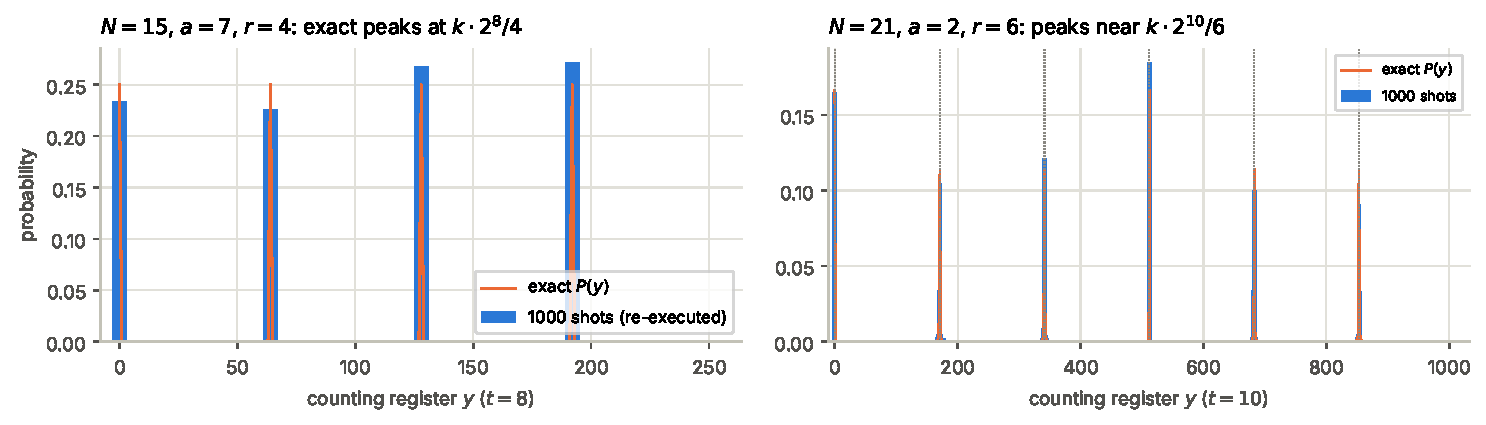
\includegraphics[width=\linewidth]{histograms.pdf}
  \small Left: the recorded default run of \texttt{Shor.ipynb} ($N = 15$, $a = 7$, seed 42) --- re-executed for this lecture with
  \numreproduced: counts $272, 268, 234, 226$ at $y = 192, 128, 0, 64$. Right: $N = 21$, $a = 2$ with the same circuit builder.
  {\color{qgrey}\scriptsize CPU simulation (\texttt{qpp-cpu}); no quantum hardware.}
\end{frame}

% =====================================================================================
\section{Module 11: Circuit architecture}
\begin{frame}[label=fBlocks]{Block diagram of Shor's algorithm}
  \centering
  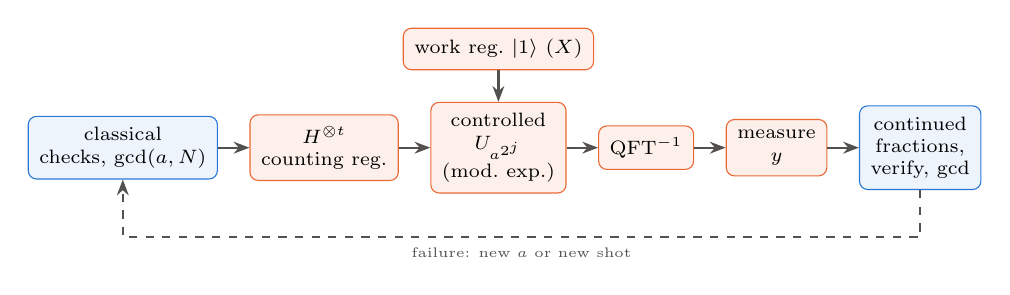
\begin{tikzpicture}[node distance=3mm and 4mm]
    \node[box] (pre) {classical\\ checks, $\gcd(a, N)$};
    \node[qbox, right=of pre] (h) {$H^{\otimes t}$\\ counting reg.};
    \node[qbox, right=of h] (me) {controlled\\ $U_{a^{2^j}}$\\ (mod.\ exp.)};
    \node[qbox, right=of me] (qft) {$\mathrm{QFT}^{-1}$};
    \node[qbox, right=of qft] (m) {measure\\ $y$};
    \node[box, right=of m] (post) {continued\\ fractions,\\ verify, $\gcd$};
    \node[qbox, above=4mm of me] (w) {work reg.\ $\ket1$ ($X$)};
    \draw[arr] (pre) -- (h); \draw[arr] (h) -- (me); \draw[arr] (me) -- (qft); \draw[arr] (qft) -- (m); \draw[arr] (m) -- (post); \draw[arr] (w) -- (me);
    \draw[arr, dashed] (post.south) -- ++(0,-0.6) -| node[pos=0.25, below, font=\tiny]{failure: new $a$ or new shot} (pre.south);
  \end{tikzpicture}\\[4pt]
  \small {\color{qorange}\textbf{orange}}: quantum (simulated here); {\color{qblue}\textbf{blue}}: classical. Cost is dominated by the
  \key{modular exponentiation}: $t = 2n$ controlled multiplications of $n$-bit numbers.
\end{frame}

\begin{frame}[label=fRegSize]{Register sizes, ancillas and scaling}
  \begin{columns}[T]
    \begin{column}{0.5\textwidth}
      \small
      \begin{itemize}\itemsep1pt
        \item counting: $t = 2n$ qubits ($2^t \ge N^2$; minimum $\lceil2\log_2N\rceil$)
        \item work: $n$ qubits
        \item \key{ancillas}: real arithmetic needs extra qubits (carries, temporary results): Beauregard $2n + 3$ in total with one recycled control qubit
        \item idealised matrix multipliers (notebook): no ancillas, $3n$ qubits
      \end{itemize}
    \end{column}
    \begin{column}{0.46\textwidth}
      \centering
      \resizebox{\linewidth}{!}{% GENERATED by make_figures.py - do not edit
\begin{tabular}{rrrrr}\toprule
bits $n$ & notebook $3n$ & Beauregard $2n+3$ & Gidney--Eker\aa{} & state vector ($3n$) \\ \midrule
4 & 12 & 11 & 13 & 65.5 kB \\
8 & 24 & 19 & 25 & 268 MB \\
16 & 48 & 35 & 49 & $10^{16}$ B \\
64 & 192 & 131 & 193 & $10^{59}$ B \\
256 & 768 & 515 & 773 & $10^{232}$ B \\
1024 & 3072 & 2051 & 3093 & $10^{926}$ B \\
2048 & 6144 & 4099 & 6190 & $10^{1851}$ B \\
\bottomrule
\end{tabular}
}\\[2pt]
      \scriptsize Logical qubits from the notebook's formulas; state-vector memory $16\cdot2^{3n}$ bytes.
    \end{column}
  \end{columns}
\end{frame}

\begin{frame}[label=fModMul]{Modular multiplication circuits}
  \begin{columns}[T]
    \begin{column}{0.5\textwidth}
      \small
      \key{Notebook} \tagimpl: each $U_c$ is one exact $2^n\times2^n$ permutation matrix (\texttt{mulmod\_matrix}), registered as a custom gate.
      Fine for simulation; \hl{not executable on hardware}.\\[4pt]
      \key{Gate level} \tagtheory: $\ket y \mapsto \ket{cy \bmod N}$ built from
      \begin{itemize}\itemsep0pt
        \item modular adders (ripple-carry or QFT-based)
        \item controlled multiply--accumulate, then uncompute with $c^{-1}$
        \item cost $O(n^2)$ gates per multiplier, $O(n^3)$ in total
      \end{itemize}
    \end{column}
    \begin{column}{0.46\textwidth}
      \begin{exampleblock}{\tagillus{} special case $N = 15$}
        \small multiplication by $2$ is a cyclic \key{bit rotation} of the 4 work bits; by $7 = -8$: three rotations plus $X$ on every bit (valid for $y = 1, \dots, 14$).
        Controlled: controlled SWAPs (Fredkin) and CNOTs.
      \end{exampleblock}
      \scriptsize Fredkin $= \mathrm{CX}\cdot\mathrm{Toffoli}\cdot\mathrm{CX}$ $= 8$ CNOTs. Such shortcuts exist only because $N = 15$ is special --- they do not generalise.
    \end{column}
  \end{columns}
\end{frame}

\begin{frame}[label=fGateLevel]{Gate-level circuit for $N = 15$ \tagillus}
  \begin{columns}[T]
    \begin{column}{0.5\textwidth}
      \small
      $t = 3$ counting $+$ 4 work qubits ($r = 4$ divides $2^3$, so 3 counting qubits suffice here):
      \begin{itemize}\itemsep1pt
        \item controlled $\times7$: 9 Fredkins $+$ 4 CNOTs $= 76$ CNOTs
        \item controlled $\times4$: 6 Fredkins $= 48$ CNOTs
        \item inverse QFT: 1 SWAP (3 CNOTs) $+$ 3 controlled phases
      \end{itemize}
      Total \numglcx{} CNOTs, \numgloneq{} one-qubit gates, \numglgates{} gates (CUDA-Q \texttt{estimate\_resources}).
    \end{column}
    \begin{column}{0.46\textwidth}
      \begin{block}{Checked}
        \small the gate-level multipliers equal the notebook's permutation matrices on all relevant inputs, and the counting distribution
        $(\frac14, 0, \frac14, 0, \frac14, 0, \frac14, 0)$ agrees with the matrix-gate circuit to $\numgatelevelagree$.
      \end{block}
      \scriptsize\color{qgrey} The multiplier constants use the known order (they skip $c = 1$); this is a \emph{teaching} circuit, not evidence of a speed-up.
    \end{column}
  \end{columns}
\end{frame}

\begin{frame}[label=fDepth]{Gate count, depth and connectivity}
  \begin{columns}[T]
    \begin{column}{0.5\textwidth}
      \small
      \key{Recorded} \tagrec{} ($N = 15$, $t = 8$, 12 qubits):
      \begin{itemize}\itemsep0pt
        \item $\numgatesfifteen$ gates without measurement: 8+8 $H$, 1 $X$, 4 SWAP, $\numcrfifteen$ \texttt{cr1}, $\numcustomfifteen$ controlled custom multipliers
        \item depth $\numdepthfifteen$
      \end{itemize}
      These counts treat a whole multiplier as \emph{one} gate --- real circuits are much larger.
    \end{column}
    \begin{column}{0.46\textwidth}
      \begin{block}{Connectivity}
        \small Controlled multipliers couple every counting qubit with the whole work register; on hardware with nearest-neighbour connectivity
        SWAP networks add depth. Surface-code architectures use lattice surgery for long-range gates.
      \end{block}
      \scriptsize As $N$ grows: qubits $\propto n$, gates $\propto n^3$ (schoolbook), depth $\propto n^3$ or less with parallel arithmetic.
    \end{column}
  \end{columns}
\end{frame}

% =====================================================================================
\section{Module 12: Implementation in CUDA-Q}
\begin{frame}[label=fEnv]{Environment and framework}
  \begin{columns}[T]
    \begin{column}{0.52\textwidth}
      \small
      \begin{itemize}\itemsep2pt
        \item \key{CUDA-Q} \numcudaqversion{} (Python), NumPy, \texttt{fractions}, \texttt{math} --- all installed and used.
        \item \texttt{BACKEND} in \texttt{Shor.ipynb}: \texttt{auto}, \texttt{cpu}, \texttt{gpu}, \texttt{multi-gpu} (state-vector or density-matrix simulators); \texttt{hardware} is \hl{refused}. The recorded run used \texttt{qpp-cpu}.
        \item \key{Qiskit / Qiskit Aer}: not installed in this repository and not used. The algorithm itself is framework-independent; a Qiskit version would need its own
              gate-level or matrix-based multipliers.
      \end{itemize}
    \end{column}
    \begin{column}{0.44\textwidth}
      \begin{block}{Notebook parameters}
        \scriptsize
        \begin{tabular}{@{}ll@{}}
          \texttt{N\_TO\_FACTOR} & 15\\
          \texttt{BASE\_A} & 7 (\texttt{None}: random)\\
          \texttt{NUM\_COUNTING\_QUBITS} & \texttt{None} ($2n$)\\
          \texttt{SHOTS} & 1000\\
          \texttt{SEED} & 42\\
          \texttt{MAX\_SIMULATION\_QUBITS} & 26
        \end{tabular}
      \end{block}
    \end{column}
  \end{columns}
\end{frame}

\begin{frame}[fragile,label=fCode1]{Circuit creation: registers, Hadamards, modular exponentiation \tagimpl}
\begin{lstlisting}[basicstyle=\ttfamily\fontsize{6.5}{7.6}\selectfont]
def mulmod_matrix(c, modulus, n):            # |y> -> |c*y mod N>, identity for y >= N
    dim = 2 ** n
    matrix = np.zeros((dim, dim))
    for y in range(dim):
        matrix[(c * y) % modulus if y < modulus else y, y] = 1.0
    return matrix

kernel = cudaq.make_kernel()
count = kernel.qalloc(t)                      # counting register
work = kernel.qalloc(n)                       # work register
kernel.x(work[n - 1])                         # |1>: last qubit = least significant bit
kernel.h(count)                               # uniform superposition
for j in range(t):
    c = pow(a, 2 ** j, modulus)               # a^(2^j) mod N, classical repeated squaring
    if c == 1:
        continue                              # identity: nothing to apply
    name = f"mulmod_{c}_mod_{modulus}"
    if name not in registered_ops:
        cudaq.register_operation(name, mulmod_matrix(c, modulus, n))
        registered_ops.add(name)
    getattr(kernel, name)(count[t - 1 - j],   # first argument = control
                          *[work[i] for i in range(n)])
\end{lstlisting}
  \scriptsize\color{qgrey} Abridged from \texttt{build\_shor\_kernel} in \texttt{Shor.ipynb}. \texttt{count[0]} is the most significant bit of $y$.
\end{frame}

\begin{frame}[fragile,label=fCode2]{Inverse QFT, measurement and sampling \tagimpl}
  \begin{columns}[T]
    \begin{column}{0.56\textwidth}
\begin{lstlisting}
for j in range(t // 2):
    kernel.swap(count[j], count[t - 1 - j])
for jj in range(t):
    j = t - 1 - jj
    for kk in range(t - 1 - j):
        k = t - 1 - kk
        kernel.cr1(-np.pi / 2 ** (k - j),
                   count[k], count[j])
    kernel.h(count[j])
kernel.mz(count)            # counting register only

counts = cudaq.sample(kernel, shots_count=SHOTS)
for bits, c in counts.items():
    y = int(bits, 2)        # MSB first
    fraction, orders = candidate_orders(y, t, N, a)
\end{lstlisting}
    \end{column}
    \begin{column}{0.4\textwidth}
      \small
      \begin{itemize}\itemsep1pt
        \item \texttt{cr1}: controlled $R_1(\lambda)$ with negative angles (inverse QFT)
        \item only the counting register is measured
        \item each distinct $y$ is post-processed; then $\gcd$ and the check $p\cdot q = N$
        \item if no shot yields factors, a new random $a$ is tried
      \end{itemize}
    \end{column}
  \end{columns}
\end{frame}

\begin{frame}[label=fVerify]{Factor verification and reproducibility}
  \small
  \begin{columns}[T]
    \begin{column}{0.5\textwidth}
      \begin{itemize}\itemsep2pt
        \item The notebook compares the result with \key{trial division} and the order with a brute-force \texttt{classical\_order} (feasible only for tiny $N$).
        \item Final report: ``\texttt{Verification p x q == N : CORRECT}'', ``\texttt{Order r found / classical check : 4 / 4}''.
        \item Fixed \texttt{SEED = 42}: re-running gives the same counts (\numreproduced).
      \end{itemize}
    \end{column}
    \begin{column}{0.46\textwidth}
      \begin{block}{Independent checks for this package}
        \scriptsize \texttt{make\_figures.py} re-executes the notebook's builder; \texttt{verify\_answers.py} recomputes all exam answers with exact
        arithmetic and compares CUDA-Q state vectors for $N = 15, 21, 33, 39$ with a NumPy formula for $P(y)$.
      \end{block}
    \end{column}
  \end{columns}
\end{frame}

% =====================================================================================
\section{Module 13: Simulation and performance}
\begin{frame}[label=fSimTypes]{Kinds of ``running'' Shor's algorithm}
  \footnotesize
  \begin{center}
  \begin{tabular}{p{0.2\linewidth}p{0.45\linewidth}p{0.25\linewidth}}
    \toprule \textbf{kind} & \textbf{what is computed} & \textbf{in this package} \\ \midrule
    mathematical & orders, peaks, probabilities by hand / exact formulas & worked examples \\
    state vector & all $2^q$ amplitudes, exact $P(y)$ & \tagillus{} (\texttt{get\_state}) \\
    shot-based & samples $y$ from the circuit & \tagrec{} \tagillus{} (\texttt{sample}) \\
    ideal & no errors & all of the above \\
    noisy & density matrix with a noise model & \tagillus{} gate-level $N = 15$ \\
    hardware & a physical quantum processor & \hl{not performed} \\ \bottomrule
  \end{tabular}
  \end{center}
  \small Simulation proves that the \emph{circuit} is correct; it does not demonstrate any quantum speed-up --- the simulator itself does exponential work.
\end{frame}

\begin{frame}[label=fRecorded]{Recorded run of \texttt{Shor.ipynb} \tagrec}
  \begin{columns}[T]
    \begin{column}{0.5\textwidth}
      \footnotesize
      \begin{tabular}{@{}ll@{}}
        \toprule CUDA-Q / target & 0.16.0 / \texttt{qpp-cpu} (fp64)\\
        GPUs visible & 0\\
        $N$, $a$ & 15, 7\\
        qubits & 8 counting $+$ 4 work $= 12$\\
        gates / depth & 51 (+ 8 \texttt{mz}) / 20\\
        shots & 1000\\
        counts $y$:\,$n_y$ & 192:\,272, 128:\,268,\\ & 0:\,234, 64:\,226\\
        success fraction & 0.766 (exact 0.75)\\
        result & $15 = 3\times5$, $r = 4$ (checked)\\ \bottomrule
      \end{tabular}
    \end{column}
    \begin{column}{0.46\textwidth}
      \footnotesize
      \begin{tabular}{@{}ll@{}}
        \toprule construction & 0.0029 s\\
        compilation (MLIR + JIT) & 0.0353 s\\
        quantum execution & 0.0179 s\\
        whole cell & 0.073 s\\
        peak host RAM & 0.87 GB\\
        process RSS & 0.55 GB\\
        state vector & $16\cdot2^{12} = 65.5$ kB\\ \bottomrule
      \end{tabular}\\[4pt]
      \scriptsize\color{qgrey} Times are for one laptop-class CPU run and vary between runs and machines; they are not a benchmark of quantum hardware.
    \end{column}
  \end{columns}
\end{frame}

\begin{frame}[label=fCases]{Further cases with the notebook's circuit \tagillus}
  \centering
  \resizebox{\linewidth}{!}{% GENERATED by make_figures.py - do not edit
\begin{tabular}{rrrcrrrrl}\toprule
$N$ & $a$ & $r$ & qubits & $U$ gates & distinct $y$ (1000 shots) & $P_{\text{succ}}$ exact & from 1000 shots & factors \\ \midrule
15 & 7 & 4 & 8 + 4 = 12 & 2 & 4 & 0.750 & 0.766 & $3\times5$ \\
15 & 2 & 4 & 8 + 4 = 12 & 2 & 4 & 0.750 & 0.766 & $3\times5$ \\
15 & 14 & 2 & 8 + 4 = 12 & 1 & 2 & 0.000 & 0.000 & none \\
21 & 2 & 6 & 10 + 5 = 15 & 10 & 54 & 0.817 & 0.822 & $3\times7$ \\
35 & 3 & 12 & 12 + 6 = 18 & 12 & 76 & 0.904 & 0.897 & $5\times7$ \\
\bottomrule
\end{tabular}
}\\[4pt]
  \small $P_{\text{succ}}$: probability that one shot yields the factors (exact, from the state vector) and the fraction observed in 1000 shots (seed 42).
  $a = 14$ \hl{always fails} ($14 \equiv -1$). $N = 35$ (18 qubits) took $\numtimethirtyfivethree$\,s on the CPU.
\end{frame}

\begin{frame}[label=fNoise]{Noisy simulation of the gate-level $N = 15$ circuit \tagillus}
  \centering
  \resizebox{0.92\linewidth}{!}{% GENERATED by make_figures.py - do not edit
\begin{tabular}{rrrrrrrrrr}\toprule
$p$ & $y=0$ & $y=1$ & $y=2$ & $y=3$ & $y=4$ & $y=5$ & $y=6$ & $y=7$ & $P_{\text{succ}}$ \\ \midrule
0 & 0.250 & 0.000 & 0.250 & 0.000 & 0.250 & 0.000 & 0.250 & 0.000 & 0.750 \\
0.001 & 0.256 & 0.001 & 0.243 & 0.001 & 0.253 & 0.001 & 0.243 & 0.001 & 0.740 \\
0.003 & 0.262 & 0.003 & 0.234 & 0.003 & 0.257 & 0.003 & 0.234 & 0.003 & 0.726 \\
0.01 & 0.258 & 0.010 & 0.225 & 0.010 & 0.254 & 0.010 & 0.224 & 0.010 & 0.703 \\
0.03 & 0.226 & 0.027 & 0.220 & 0.027 & 0.226 & 0.027 & 0.220 & 0.027 & 0.665 \\
\bottomrule
\end{tabular}
}\\[4pt]
  \small \texttt{density-matrix-cpu}; depolarizing channel $p$ after every $H$, $R_z$, $X$ and two-qubit depolarizing $p$ after every CNOT and controlled phase
  (\numglcx{} CNOTs). Success falls from $\numglsucc$ towards the random-outcome baseline $\numunifsucc$: $\numnoisesuccone$ at $p = 0.01$, $\numnoisesuccthree$ at $p = 0.03$.
  {\color{qgrey}\scriptsize An idealised noise model --- not a model of a specific device.}
\end{frame}

\begin{frame}[label=fApprox]{Approximate inverse QFT for $N = 21$ \tagillus}
  \begin{columns}[T]
    \begin{column}{0.42\textwidth}
      \centering
      \resizebox{\linewidth}{!}{% GENERATED by make_figures.py - do not edit
\begin{tabular}{rrr}\toprule
max.\ $k - j$ kept & controlled phases & $P_{\text{succ}}$ \\ \midrule
1 & 9 & 0.4397 \\
2 & 17 & 0.6892 \\
3 & 24 & 0.7865 \\
4 & 30 & 0.8105 \\
9 & 45 & 0.8165 \\
\bottomrule
\end{tabular}
}
    \end{column}
    \begin{column}{0.54\textwidth}
      \small
      Drop controlled phases between qubits at distance $k - j > m$ (angles $\le \pi/2^m$).
      \begin{itemize}\itemsep1pt
        \item $m = 4$: 30 instead of 45 phases, success $0.8105$ vs $0.8165$
        \item $m = 1$: only 9 phases, success drops to $0.44$
      \end{itemize}
      Asymptotically $m \approx \log_2t$ suffices, reducing the QFT to $O(t\log t)$ gates. The QFT was never the bottleneck --- modular exponentiation is.
    \end{column}
  \end{columns}
\end{frame}

% =====================================================================================
\section{Module 14: Limitations}
\begin{frame}[label=fLimits]{Practical challenges}
  \begin{columns}[T]
    \begin{column}{0.5\textwidth}
      \small
      \begin{itemize}\itemsep1pt
        \item \key{qubits}: $\approx2n$--$3n$ \emph{logical} qubits; $\approx6200$ for RSA-2048
        \item \key{gates}: billions of Toffoli gates for RSA-2048
        \item \key{error correction}: each logical qubit $\approx$ hundreds to thousands of physical qubits
        \item \key{fidelity and decoherence}: physical error rates $\sim10^{-3}$ must be suppressed below $\approx1/(\text{number of operations}) \sim 10^{-10}$ per logical operation
        \item \key{depth and connectivity}: long sequential arithmetic, routing overhead
        \item \key{classical control}: real-time decoding of error syndromes
      \end{itemize}
    \end{column}
    \begin{column}{0.46\textwidth}
      \begin{alertblock}{Small demonstrations $\neq$ RSA}
        \small Factoring $15$ or $21$ uses a handful of qubits and often a circuit simplified with \emph{the known answer} (as in our gate-level $N = 15$ circuit).
        Such ``compiled'' demonstrations do not scale and say nothing about RSA-2048.
      \end{alertblock}
      \scriptsize Classical simulation is no way out: the notebook's memory budget of 80 GB allows only $N \le 1023$ (30 qubits).
    \end{column}
  \end{columns}
\end{frame}

\begin{frame}[label=fScaling]{Why simulation and today's hardware stop early}
  \begin{columns}[T]
    \begin{column}{0.5\textwidth}
      \small
      \key{Simulation} \tagimpl{} (notebook's reverse estimation):
      \begin{itemize}\itemsep1pt
        \item 80 GB $\Rightarrow$ 32-qubit state vector $\Rightarrow$ $N \le 1023$ (10 bits)
        \item 100 logical qubits $\Rightarrow$ 33-bit $N$ ($3n$) or 48-bit $N$ ($2n + 3$)
        \item each extra bit: $3$ more qubits, $8\times$ memory
      \end{itemize}
    \end{column}
    \begin{column}{0.46\textwidth}
      \small
      \key{Hardware} \tagtheory:
      \begin{itemize}\itemsep1pt
        \item current devices: noisy physical qubits, no large-scale error correction yet
        \item gap to RSA-2048: millions of high-quality physical qubits running for hours to days
      \end{itemize}
      \scriptsize\color{qgrey} No hardware claims are made in this lecture; the notebook refuses hardware targets.
    \end{column}
  \end{columns}
\end{frame}

% =====================================================================================
\section{Module 15: Cryptography}
\begin{frame}[label=fThreat]{How Shor's algorithm threatens public-key cryptography}
  \footnotesize
  \begin{center}
  \resizebox{\linewidth}{!}{%
  \begin{tabular}{lll}
    \toprule \textbf{scheme} & \textbf{hard problem} & \textbf{quantum attack}\\ \midrule
    RSA & factoring & Shor: broken (polynomial)\\
    Diffie--Hellman, DSA & discrete log in $\mathbb Z_p^*$ & Shor: broken\\
    ECDH, ECDSA, EdDSA & elliptic-curve discrete log & Shor: broken (fewer qubits than RSA of equal strength)\\
    AES, SHA-2/3 & no algebraic period & Grover: square-root speed-up only $\Rightarrow$ use 256-bit keys\\ \bottomrule
  \end{tabular}}
  \end{center}
  \begin{block}{Theory versus practice}
    \small \key{Theoretical impact}: complete break of RSA/ECC by a large fault-tolerant quantum computer. \key{Practical capability today}: none ---
    no such machine exists. The risk is about the \emph{future}.
  \end{block}
\end{frame}

\begin{frame}[label=fPQC]{Post-quantum cryptography and NIST standards}
  \begin{columns}[T]
    \begin{column}{0.52\textwidth}
      \small
      \key{Post-quantum cryptography}: classical algorithms based on problems with no known efficient quantum algorithm (lattices, hash functions, codes).
      \begin{itemize}\itemsep1pt
        \item \key{FIPS 203} ML-KEM (Kyber) --- key encapsulation
        \item \key{FIPS 204} ML-DSA (Dilithium) --- signatures
        \item \key{FIPS 205} SLH-DSA (SPHINCS+) --- hash-based signatures
      \end{itemize}
      published by NIST in August 2024; HQC (code-based KEM) selected in 2025 as a backup.
    \end{column}
    \begin{column}{0.44\textwidth}
      \begin{alertblock}{Not to confuse}
        \small \key{Post-quantum} cryptography runs on classical computers. \key{Quantum key distribution} is a different technology that needs quantum hardware.
      \end{alertblock}
    \end{column}
  \end{columns}
\end{frame}

\begin{frame}[label=fMigration]{Quantum-safe migration: why organisations act now}
  \small
  \begin{columns}[T]
    \begin{column}{0.5\textwidth}
      \begin{itemize}\itemsep2pt
        \item \key{Harvest now, decrypt later}: encrypted traffic recorded today can be decrypted once a large quantum computer exists.
        \item \key{Mosca's inequality}: act if (data lifetime) $+$ (migration time) $>$ (time until a cryptographically relevant quantum computer).
        \item Migrations take years: inventory, hybrid key exchange (e.g.\ X25519 $+$ ML-KEM), crypto-agility.
      \end{itemize}
    \end{column}
    \begin{column}{0.46\textwidth}
      \begin{block}{Real-world implications}
        \small TLS, VPNs, code signing, PKI certificates, long-lived devices. Government roadmaps (e.g.\ NIST IR 8547, draft 2024) plan to deprecate
        quantum-vulnerable public-key algorithms by 2030 and disallow them by 2035.
      \end{block}
    \end{column}
  \end{columns}
\end{frame}

% =====================================================================================
\section{Module 16: Advanced topics}
\begin{frame}[label=fHSP]{Order finding, phase estimation and the hidden subgroup problem}
  \small
  \begin{itemize}\itemsep2pt
    \item Order finding is an instance of the \key{abelian hidden subgroup problem}: find the subgroup $r\mathbb Z$ on which $f(x) = a^x$ is constant.
    \item The same Fourier-sampling method solves \key{discrete logarithms} (two-dimensional period of $g^xh^{-y}$) and Simon's problem.
    \item \key{Ekerå--Håstad} variants factor RSA moduli via a short discrete logarithm with fewer qubits; \key{Regev (2023)} proposed a
          multidimensional variant with $\approx n^{1.5}$ gates per run but more runs and qubits.
    \item Non-abelian generalisations (graph isomorphism, lattice problems) have \hl{no} known efficient algorithm --- the basis of post-quantum security.
  \end{itemize}
\end{frame}

\begin{frame}[label=fSemiclassical]{Approximate and semiclassical QFT}
  \begin{columns}[T]
    \begin{column}{0.5\textwidth}
      \small
      \key{Approximate QFT} (Coppersmith 1994): omit rotations by angles $< \pi/2^m$; $O(t\log t)$ gates, small error (see Module 13).\\[4pt]
      \key{Semiclassical QFT} (Griffiths--Niu 1996): measure the counting qubits one at a time and apply the remaining rotations \hl{classically controlled}.
      One physical control qubit is \key{recycled} $2n$ times.
    \end{column}
    \begin{column}{0.46\textwidth}
      \begin{block}{Consequence}
        \small qubits $3n \to 2n + 3$ (Beauregard 2003: $n$ work, $n + 1$ for a QFT-based adder, 1 ancilla, 1 control). Same measurement statistics;
        needs mid-circuit measurement and fast feed-forward.
      \end{block}
    \end{column}
  \end{columns}
\end{frame}

\begin{frame}[label=fFT]{Fault tolerance: logical versus physical qubits}
  \begin{columns}[T]
    \begin{column}{0.52\textwidth}
      \small
      \begin{itemize}\itemsep1pt
        \item \key{Physical qubit}: noisy hardware element (error $\sim10^{-3}$).
        \item \key{Logical qubit}: encoded in many physical qubits, e.g.\ a \key{surface code} patch of distance $d$ ($\approx2d^2$ qubits).
        \item Logical error $\sim(p/p_{\text{th}})^{(d+1)/2}$: grows exponentially better with $d$ below threshold $p_{\text{th}} \approx 1\%$.
        \item Clifford gates are cheap; $T$/Toffoli gates need \key{magic states} (distillation or cultivation) --- they dominate Shor's cost.
      \end{itemize}
    \end{column}
    \begin{column}{0.44\textwidth}
      \begin{block}{Published RSA-2048 estimates \tagtheory}
        \scriptsize
        \begin{tabular}{@{}lll@{}}
          \toprule & physical qubits & time\\ \midrule
          Gidney--Ekerå 2019 & $\approx20$ million & $\approx8$ h\\
          Gidney 2025 & $< 1$ million & $< 1$ week\\ \bottomrule
        \end{tabular}\\[3pt]
        assumptions: $10^{-3}$ physical error rate, $1\,\mu$s surface-code cycle. Estimates, not experiments.
      \end{block}
    \end{column}
  \end{columns}
\end{frame}

\begin{frame}[label=fResearch]{Optimised arithmetic and research directions}
  \small
  \begin{columns}[T]
    \begin{column}{0.5\textwidth}
      \key{Optimised modular exponentiation}
      \begin{itemize}\itemsep1pt
        \item windowed arithmetic and table lookups
        \item coset representation, oblivious carry runways
        \item approximate residue arithmetic (Gidney 2025)
        \item Montgomery and Karatsuba-style multipliers
      \end{itemize}
    \end{column}
    \begin{column}{0.46\textwidth}
      \key{Open directions}
      \begin{itemize}\itemsep1pt
        \item better codes (yoked surface codes, qLDPC codes)
        \item cheaper magic states
        \item elliptic-curve discrete logs (fewer qubits than RSA)
        \item honest benchmarks: avoid ``compiled'' demonstrations
      \end{itemize}
    \end{column}
  \end{columns}
  \vspace{4pt}
  \centering\color{qgrey} The trend: each new paper lowers the estimated cost --- one reason to migrate to post-quantum cryptography early.
\end{frame}

% =====================================================================================
\section{Summary}
\begin{frame}[label=fPitfalls]{Common misconceptions}
  \small
  \begin{enumerate}\itemsep1pt
    \item ``Shor tries all factors in parallel'' --- \hl{no}: one measurement gives one sample; interference does the work.
    \item ``The QFT factors $N$'' --- the QFT is a subroutine; modular exponentiation and classical steps are essential.
    \item ``The measured $y$ is the period'' --- $y/2^t \approx s/r$; continued fractions and verification are needed.
    \item ``$y = 0$ means $r = 1$'' --- $y = 0$ occurs for every $r$ and is uninformative.
    \item ``A correct order always gives factors'' --- odd $r$ or $a^{r/2} \equiv -1$ fail; repeat.
    \item ``Shor works for $N = p^k$'' --- prime powers are handled classically.
    \item ``Factoring 15 on a device shows RSA is broken'' --- tiny compiled circuits do not scale.
    \item ``Simulating Shor demonstrates quantum speed-up'' --- the simulator does exponential classical work.
  \end{enumerate}
\end{frame}

\begin{frame}[label=fSummary]{Summary}
  \begin{columns}[T]
    \begin{column}{0.5\textwidth}
      \small
      \begin{enumerate}\itemsep1pt
        \item factoring $\to$ order finding (classical reduction)
        \item order finding $=$ phase estimation of $U_a$
        \item Hadamards, controlled $U_{a^{2^j}}$, inverse QFT, measure
        \item $y/2^t \approx s/r$ $\to$ continued fractions $\to$ verify $r$
        \item $\gcd(a^{r/2} \pm 1, N)$ $\to$ factors; repeat on failure
      \end{enumerate}
    \end{column}
    \begin{column}{0.46\textwidth}
      \begin{block}{Numbers to remember}
        \scriptsize
        $N = 15$: 12 qubits, outcomes $0, 64, 128, 192$, success $3/4$\\
        $N = 21$: 15 qubits, $r = 6$, success $\approx0.82$\\
        RSA-2048: $\approx6200$ logical, $< 10^6$--$2\times10^7$ physical qubits (estimates)\\
        Post-quantum: FIPS 203/204/205
      \end{block}
    \end{column}
  \end{columns}
\end{frame}

\begin{frame}{Syllabus coverage map (1/2)}
  \scriptsize
  \begin{tabular}{p{0.3\linewidth}p{0.62\linewidth}}
    \toprule \textbf{Module} & \textbf{Slides}\\ \midrule
    1 Introduction & what it is \pageref{fWhat}, history \pageref{fHistory}, factoring vs prime factorisation \pageref{fFactoring}, classical vs quantum \pageref{fClassVsQuantum}\\
    2 Mathematical foundations & primes, gcd, Euclid \pageref{fIntegers}; modular arithmetic \pageref{fModular}; totient, order \pageref{fTotient}; modular exponentiation \pageref{fModExp}; examples \pageref{fNTExamples}\\
    3 Classical factorization & trial division \pageref{fTrial}; complexity \pageref{fComplexity}; RSA \pageref{fRSAdep}\\
    4 Core idea & reduction \pageref{fReduction}; $f(x) = a^x \bmod N$ \pageref{fPeriodic}; conditions on $r$ \pageref{fWhyEven}; exceptions \pageref{fPrimePower}\\
    5 Quantum foundations & registers \pageref{fRegisters}; superposition, parallelism \pageref{fSuperposition}; gates, reversibility \pageref{fGates}; entanglement, measurement, interference \pageref{fEntangle}\\
    6 Period finding & circuit \pageref{fPFCircuit}; states \pageref{fPFState}; exact peaks \pageref{fPFExact}; intuition \pageref{fPFIntuition}\\
    7 QFT & definition \pageref{fQFTDef}; circuit, inverse \pageref{fQFTCircuit}; peaks \pageref{fQFTPeaks}; role \pageref{fQFTRole}\\
    8 Phase estimation & eigenvectors \pageref{fEigen}; kickback \pageref{fKickback}; QPE \pageref{fQPE}; QPE = order finding \pageref{fQPEOrder}\\ \bottomrule
  \end{tabular}
\end{frame}

\begin{frame}{Syllabus coverage map (2/2)}
  \scriptsize
  \begin{tabular}{p{0.3\linewidth}p{0.62\linewidth}}
    \toprule \textbf{Module} & \textbf{Slides}\\ \midrule
    9 Continued fractions & why needed \pageref{fCFWhy}; algorithm \pageref{fCF}; worked table \pageref{fCFTable}; verification, gcd \pageref{fCFCode}\\
    10 Worked examples & $N = 15$ steps 1--4 \pageref{fEx15a}, 5--6 \pageref{fEx15b}, 7--12 \pageref{fEx15c}; $N = 21$ \pageref{fEx21}; distributions \pageref{fHist}\\
    11 Circuit architecture & blocks \pageref{fBlocks}; sizes, ancillas \pageref{fRegSize}; multipliers \pageref{fModMul}; gate level \pageref{fGateLevel}; depth, connectivity \pageref{fDepth}\\
    12 Implementation & environment \pageref{fEnv}; circuit code \pageref{fCode1}; QFT, sampling \pageref{fCode2}; verification \pageref{fVerify}\\
    13 Simulation, performance & kinds \pageref{fSimTypes}; recorded run \pageref{fRecorded}; cases \pageref{fCases}; noise \pageref{fNoise}; approximate QFT \pageref{fApprox}\\
    14 Limitations & challenges \pageref{fLimits}; scaling \pageref{fScaling}\\
    15 Cryptography & threat \pageref{fThreat}; PQC \pageref{fPQC}; migration \pageref{fMigration}\\
    16 Advanced topics & HSP, variants \pageref{fHSP}; approximate/semiclassical QFT \pageref{fSemiclassical}; fault tolerance \pageref{fFT}; research \pageref{fResearch}\\ \bottomrule
  \end{tabular}
\end{frame}

\begin{frame}{References}
  \scriptsize
  \begin{itemize}\itemsep1pt
    \item P.\ W.\ Shor, Algorithms for quantum computation: discrete logarithms and factoring, FOCS 1994; SIAM J.\ Comput.\ 26 (1997) 1484.
    \item M.\ A.\ Nielsen, I.\ L.\ Chuang, \emph{Quantum Computation and Quantum Information}, Ch.\ 5 (QFT, phase estimation, order finding).
    \item D.\ Coppersmith, An approximate Fourier transform useful in quantum factoring, IBM RC19642 (1994).
    \item R.\ B.\ Griffiths, C.-S.\ Niu, Semiclassical Fourier transform for quantum computation, PRL 76 (1996) 3228.
    \item S.\ Beauregard, Circuit for Shor's algorithm using $2n + 3$ qubits, QIC 3 (2003) 175.
    \item C.\ Gidney, M.\ Ekerå, How to factor 2048 bit RSA integers in 8 hours using 20 million noisy qubits, Quantum 5 (2021) 433.
    \item C.\ Gidney, How to factor 2048 bit RSA integers with less than a million noisy qubits, arXiv:2505.15917 (2025).
    \item J.\ A.\ Smolin, G.\ Smith, A.\ Vargo, Oversimplifying quantum factoring, Nature 499 (2013) 163.
    \item NIST FIPS 203, 204, 205 (2024). NVIDIA CUDA-Q documentation, version \numcudaqversion.
  \end{itemize}
\end{frame}

\end{document}
